\begin{figure}[htbp]
    \centering
    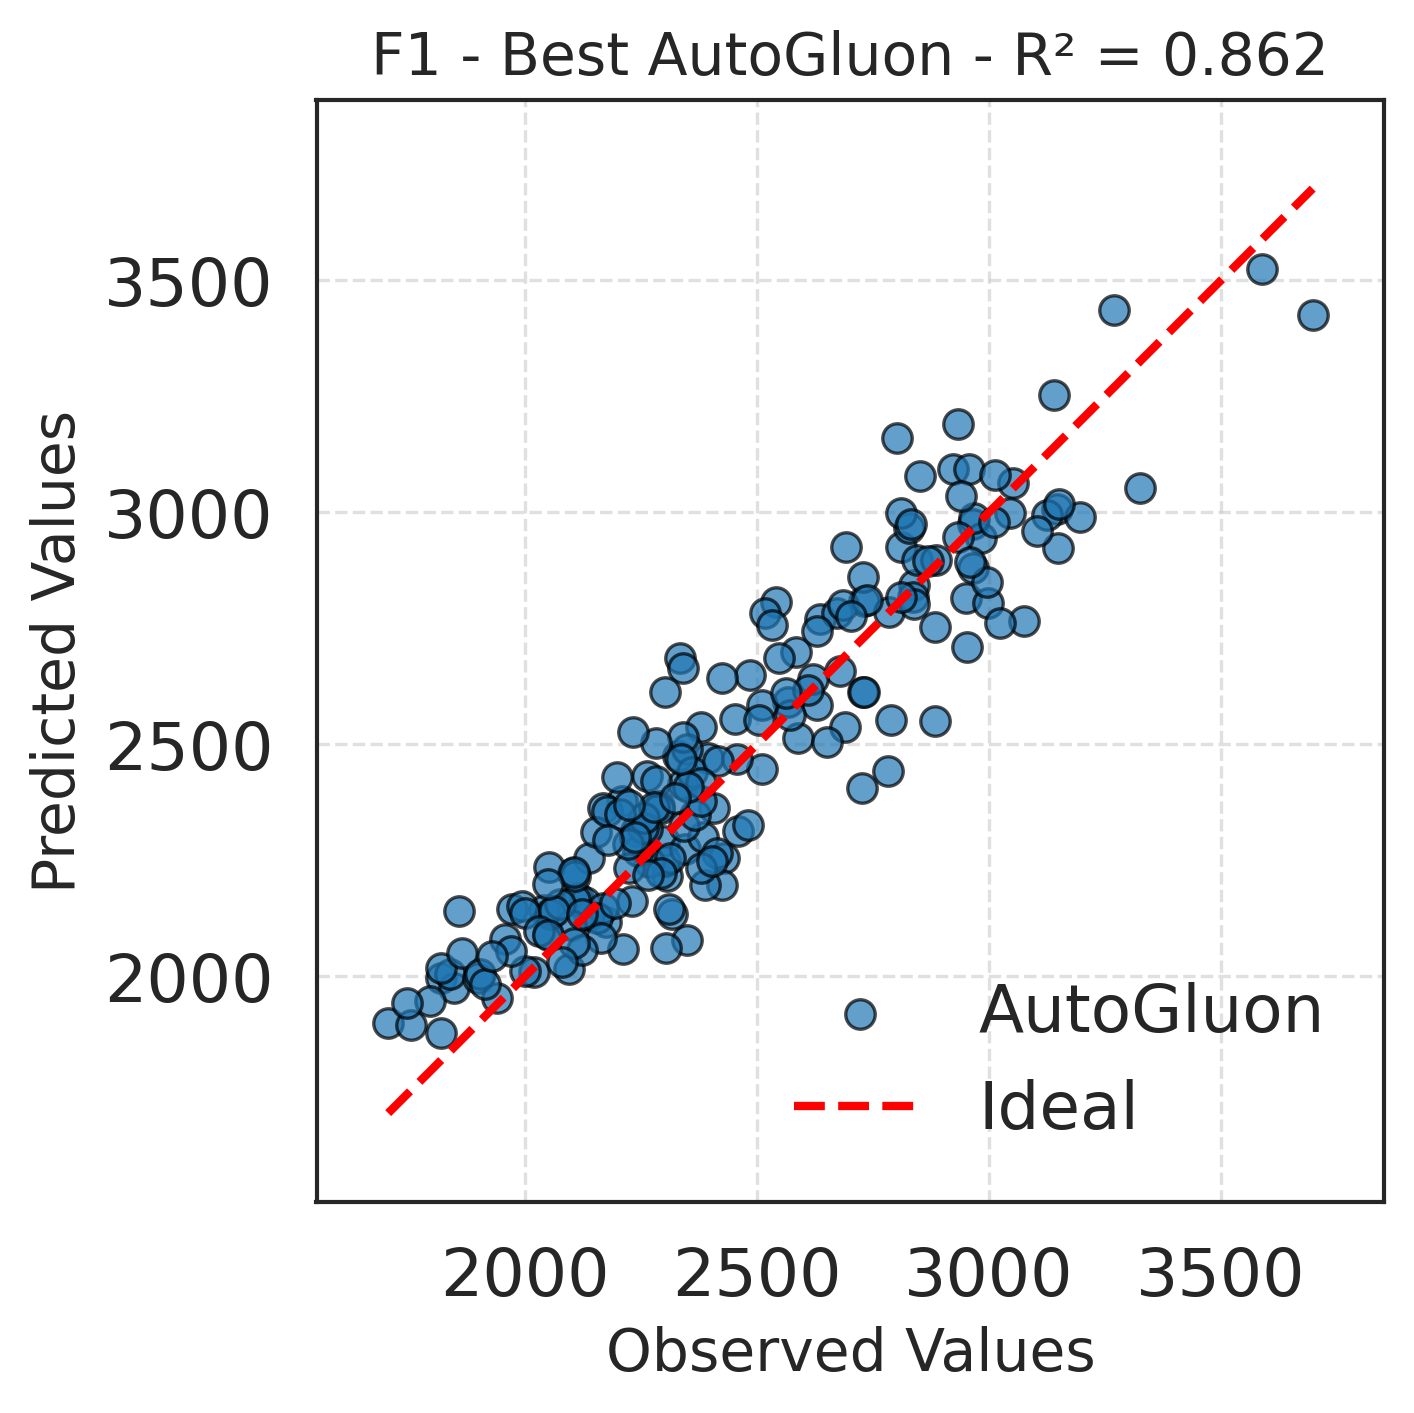
\includegraphics[width=0.8\textwidth]{./img/AutoGluon_best_scatter_F1.png}
    \caption{Autogluon Best Scatter F1}
    \label{fig:autogluon-best-scatter-f1}
\end{figure}

\begin{figure}[htbp]
    \centering
    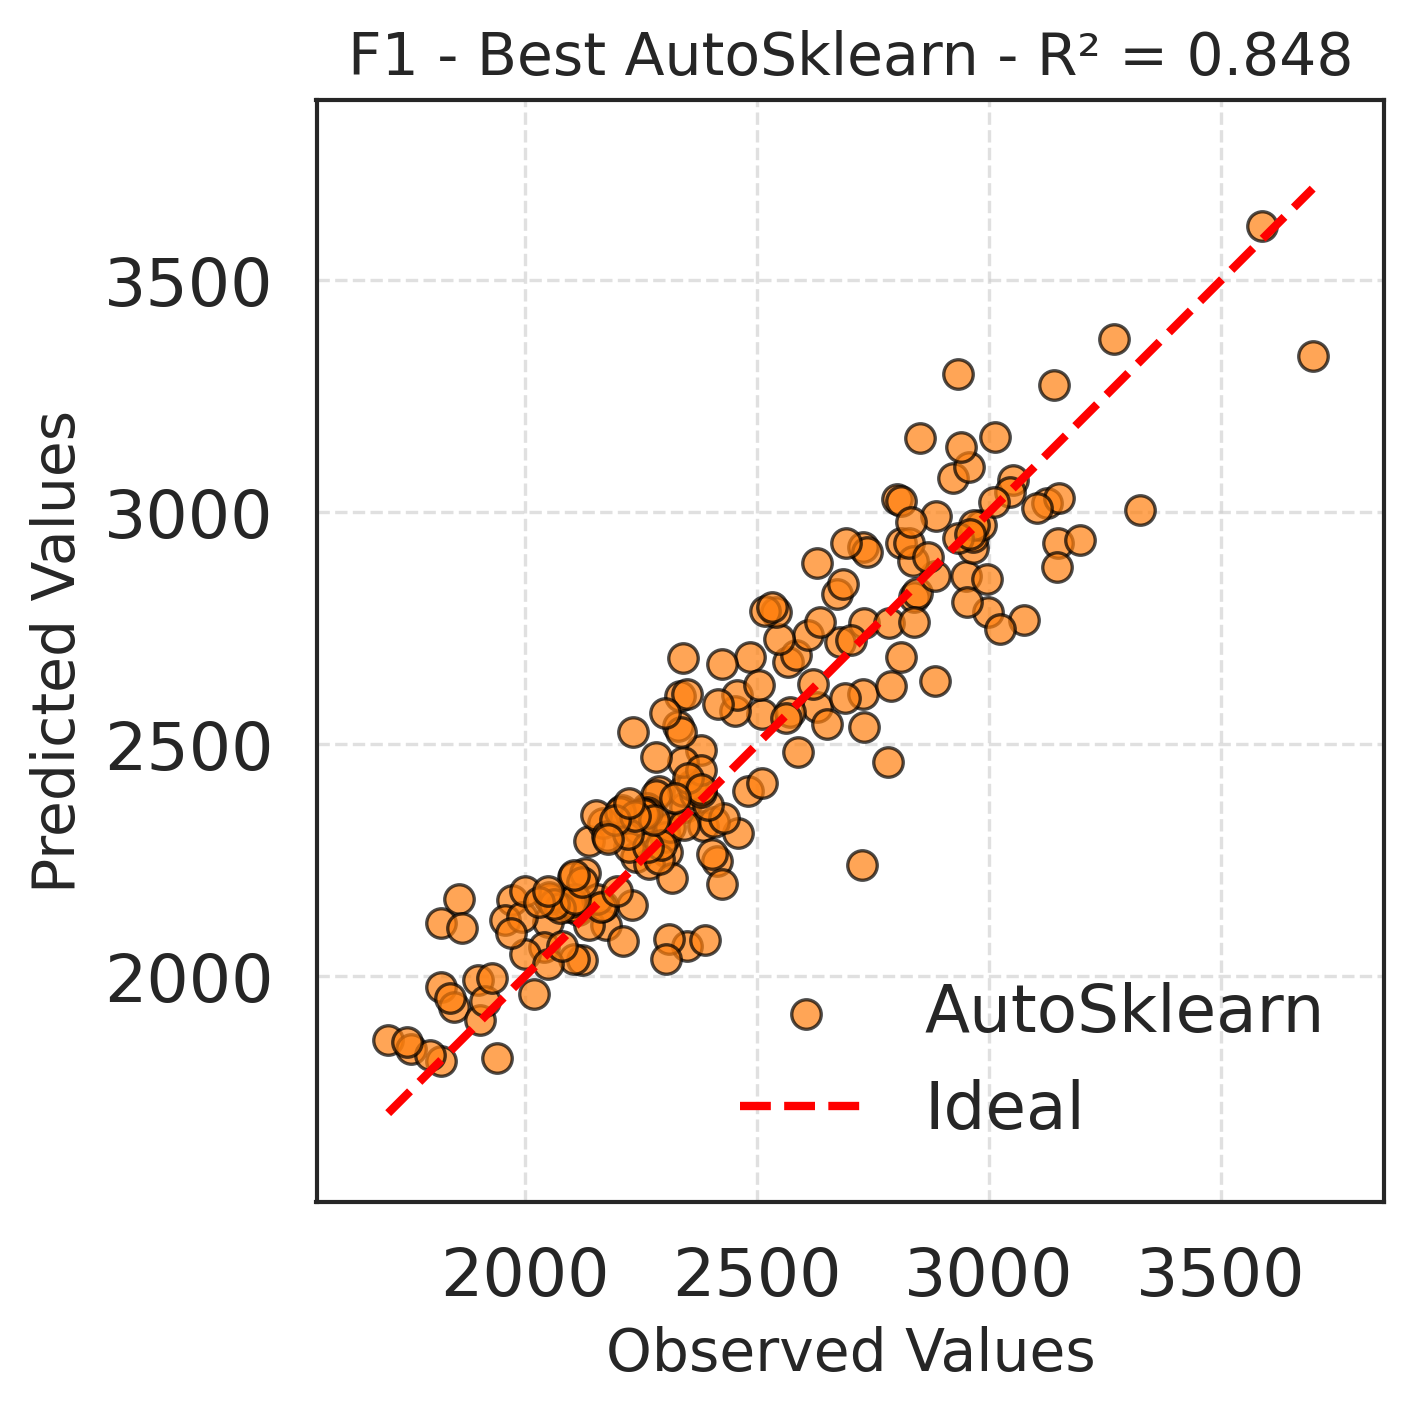
\includegraphics[width=0.8\textwidth]{./img/AutoSklearn_best_scatter_F1.png}
    \caption{Autosklearn Best Scatter F1}
    \label{fig:autosklearn-best-scatter-f1}
\end{figure}

\begin{figure}[htbp]
    \centering
    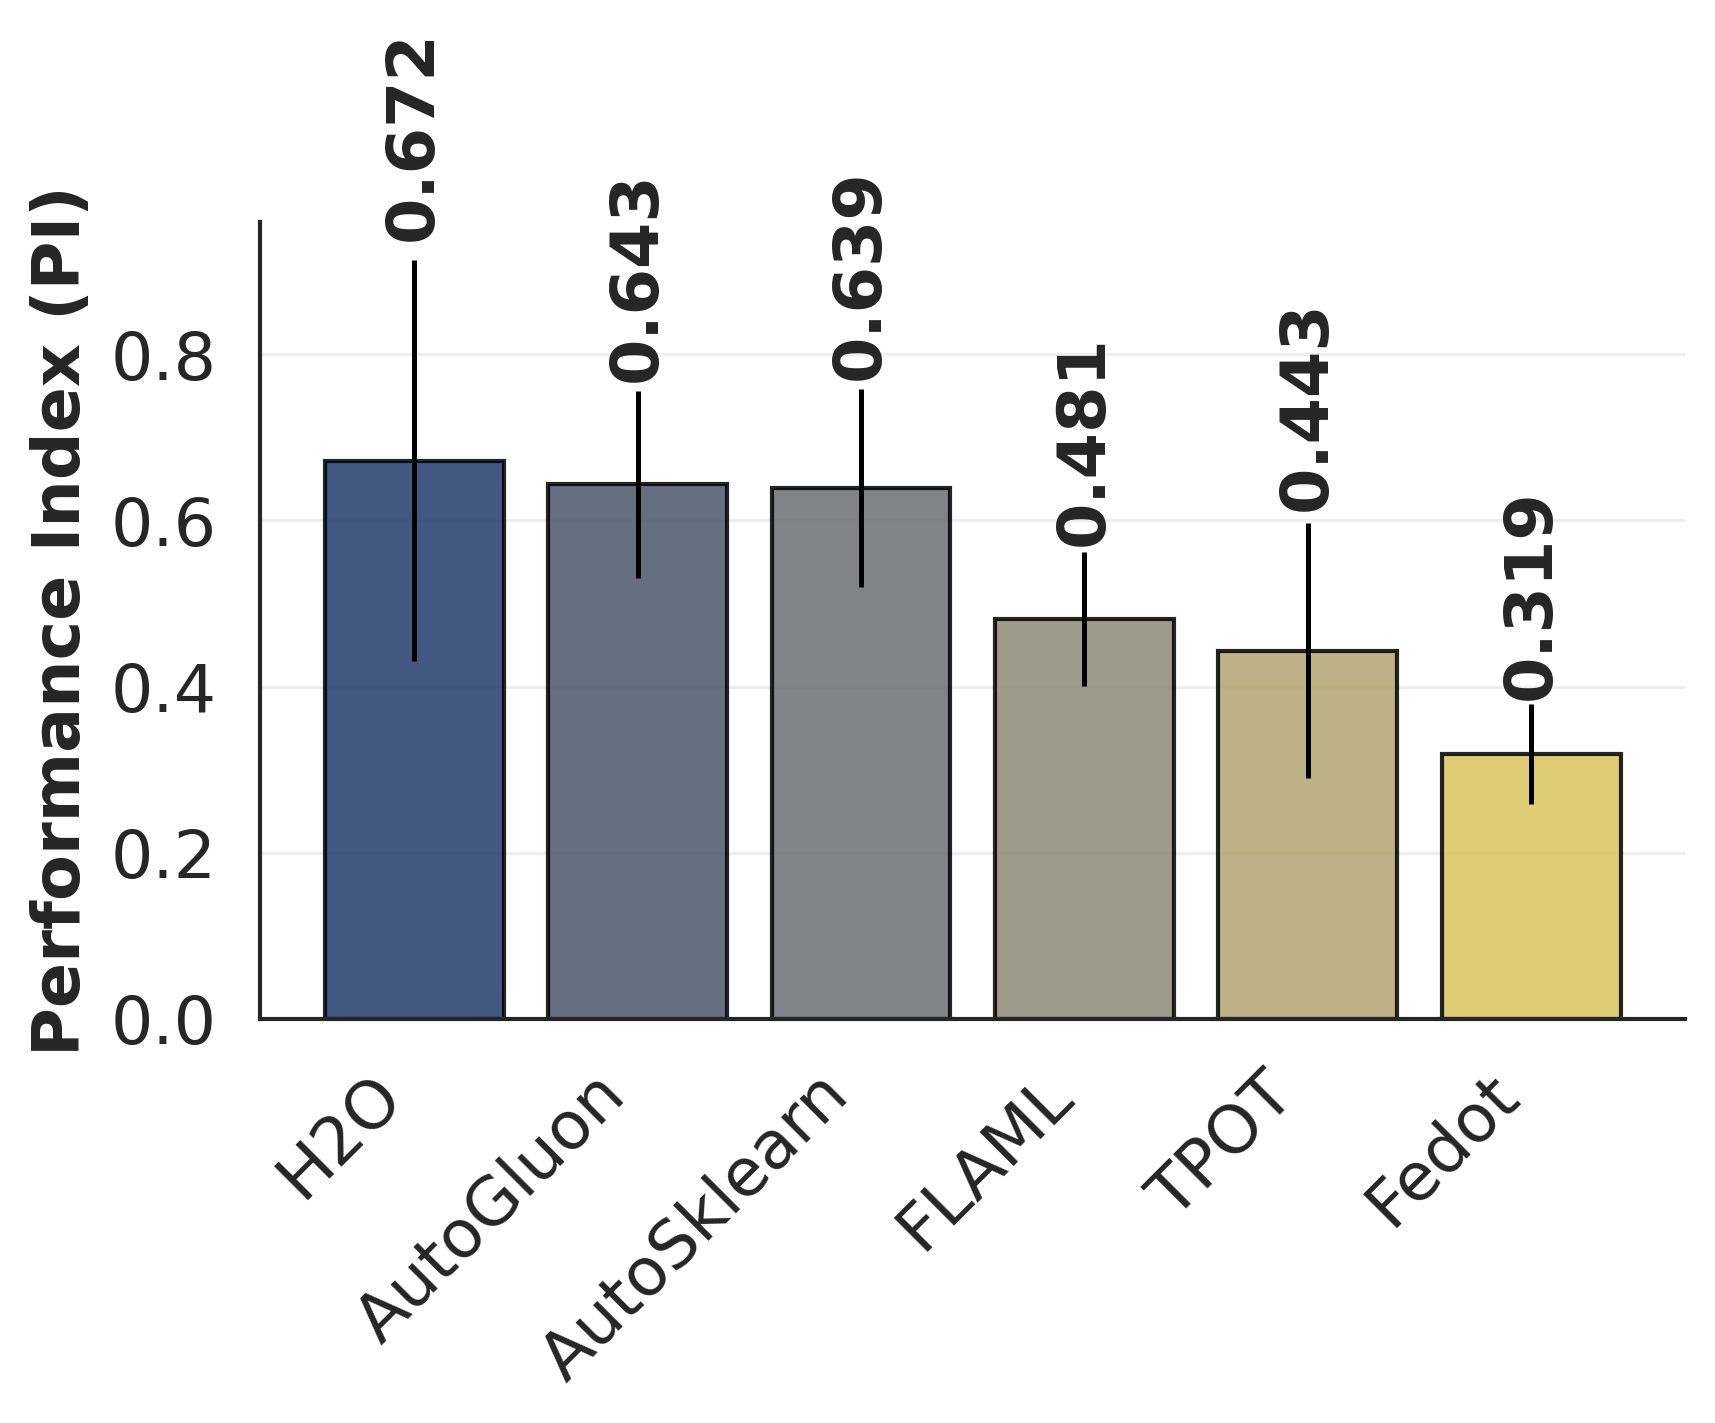
\includegraphics[width=0.8\textwidth]{./img/F1_pi.png}
    \caption{F1 Pi}
    \label{fig:f1-pi}
\end{figure}

\begin{figure}[htbp]
    \centering
    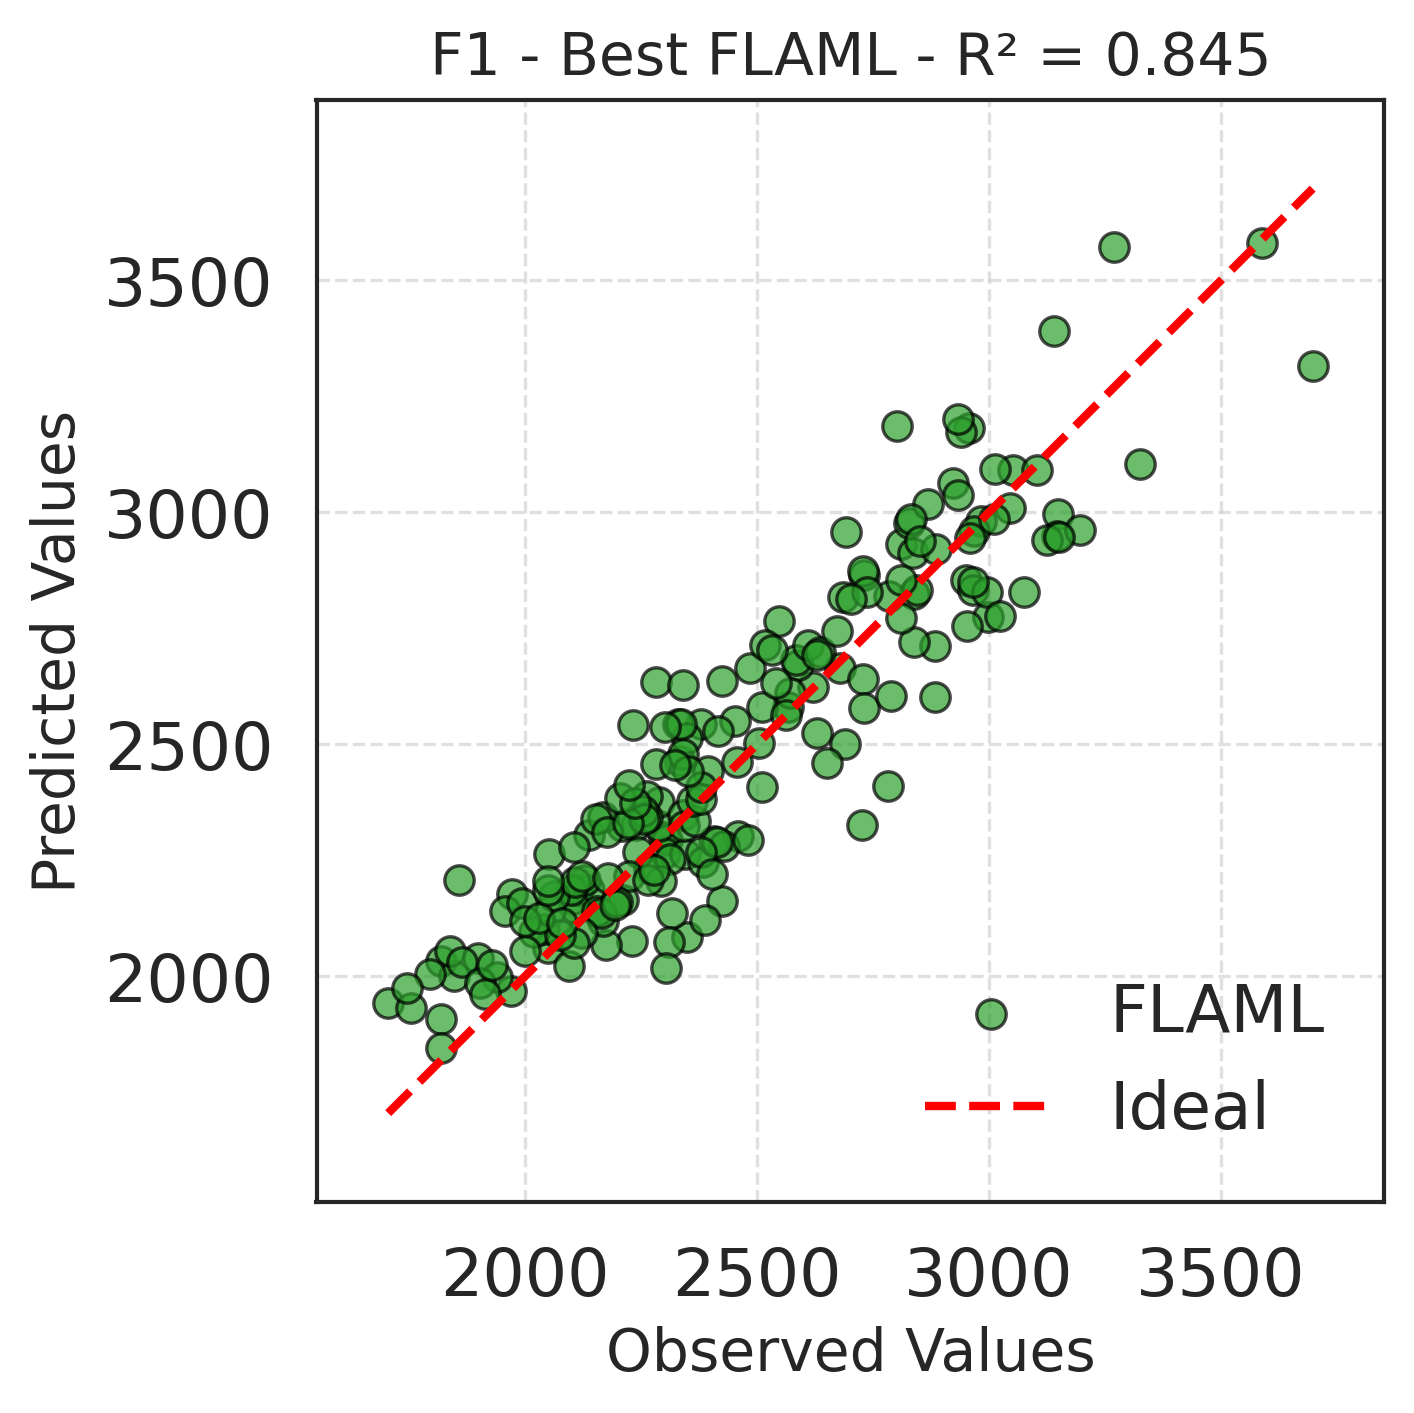
\includegraphics[width=0.8\textwidth]{./img/FLAML_best_scatter_F1.png}
    \caption{Flaml Best Scatter F1}
    \label{fig:flaml-best-scatter-f1}
\end{figure}

\begin{figure}[htbp]
    \centering
    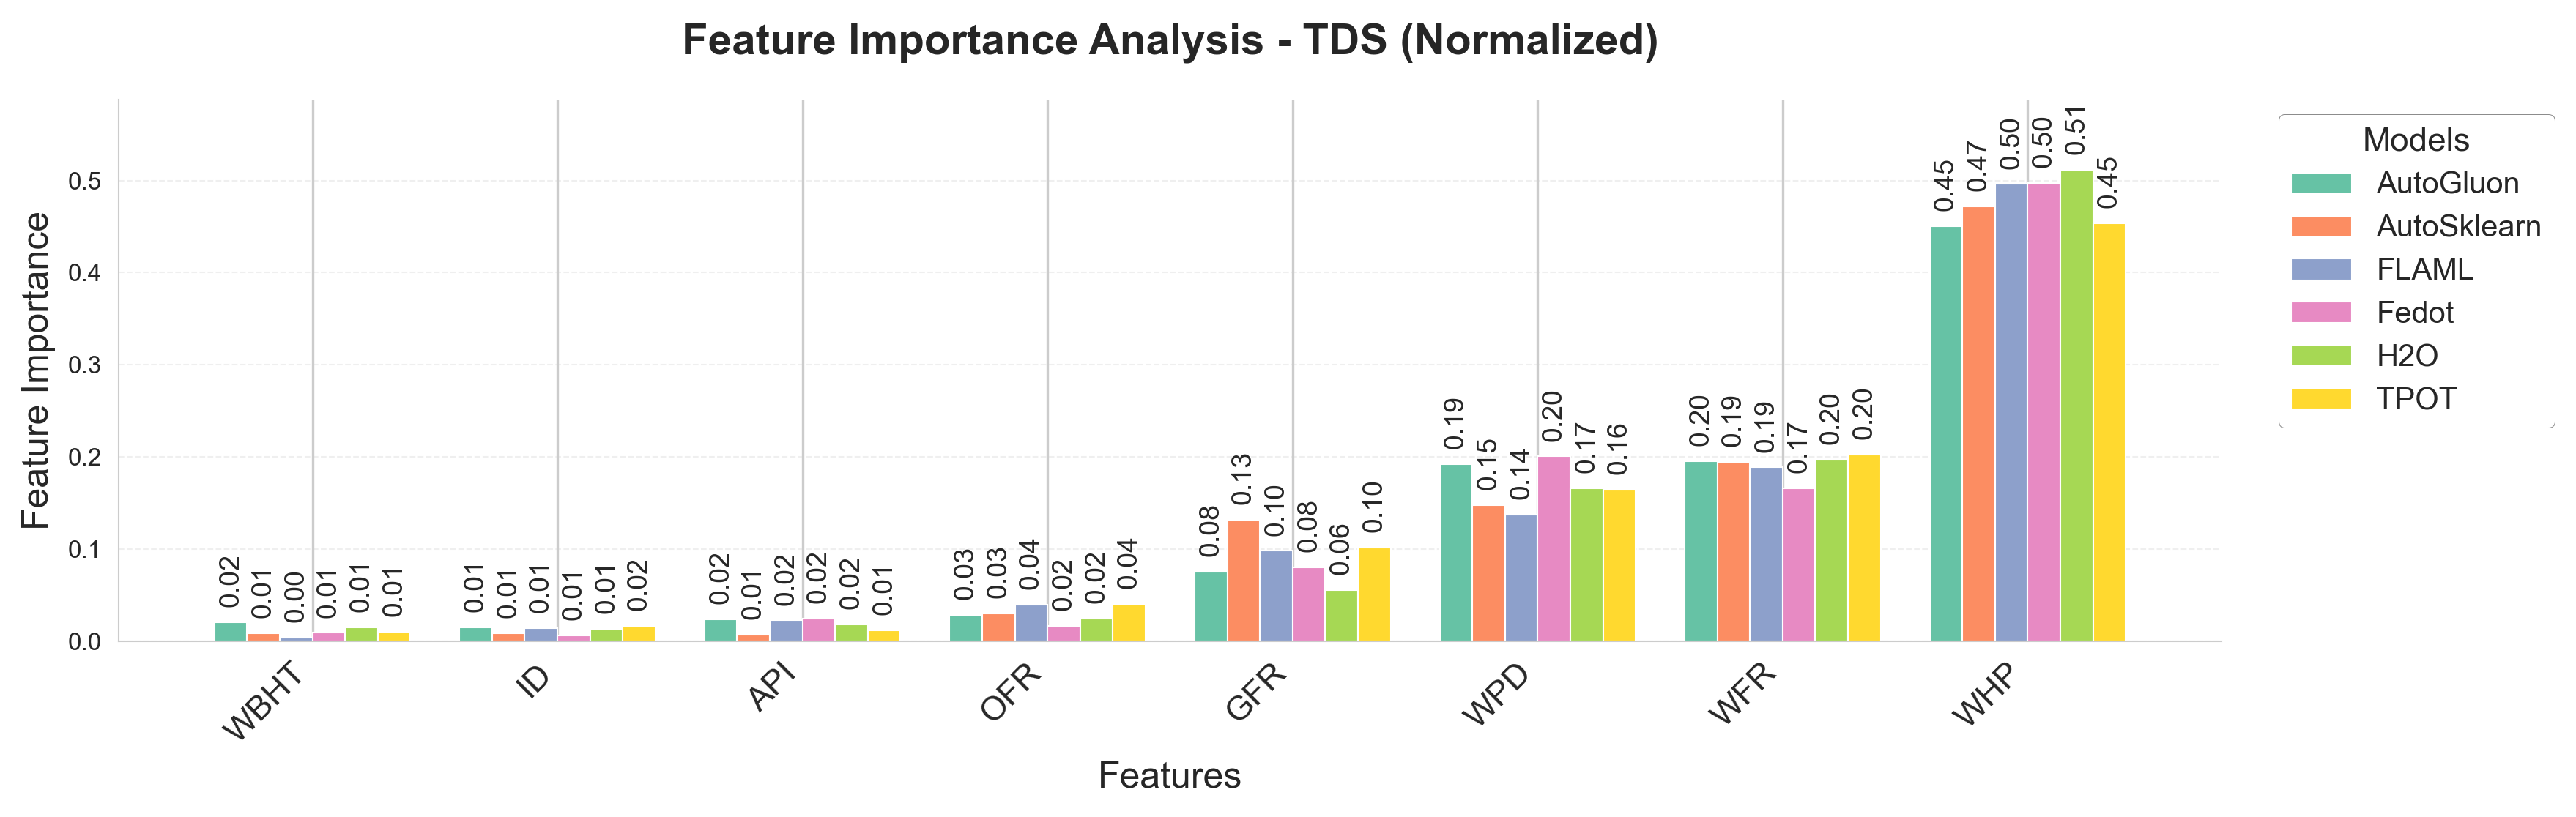
\includegraphics[width=0.8\textwidth]{./img/Feature_Importance_Feature_Importance_Analysis_-_TDS_vert.png}
    \caption{Feature Importance Feature Importance Analysis - Tds Vert}
    \label{fig:feature-importance-feature-importance-analysis---tds-vert}
\end{figure}

\begin{figure}[htbp]
    \centering
    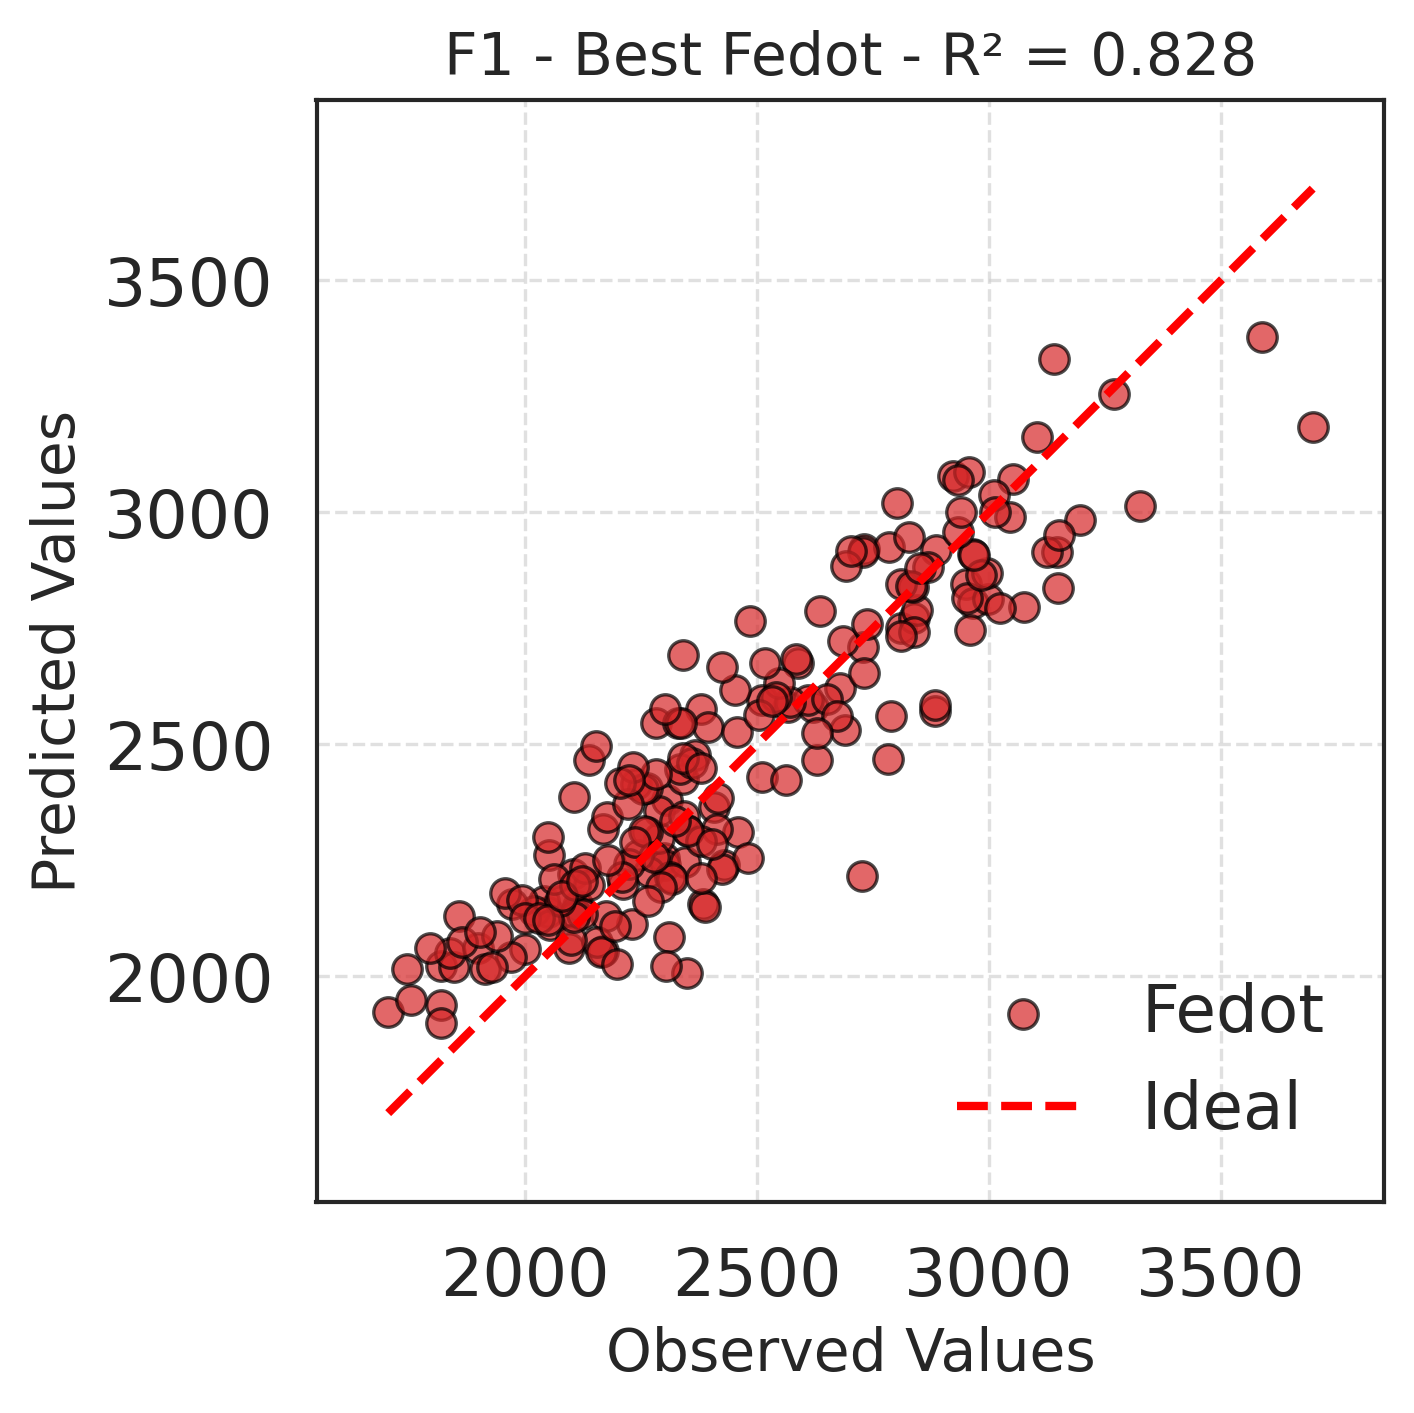
\includegraphics[width=0.8\textwidth]{./img/Fedot_best_scatter_F1.png}
    \caption{Fedot Best Scatter F1}
    \label{fig:fedot-best-scatter-f1}
\end{figure}

\begin{figure}[htbp]
    \centering
    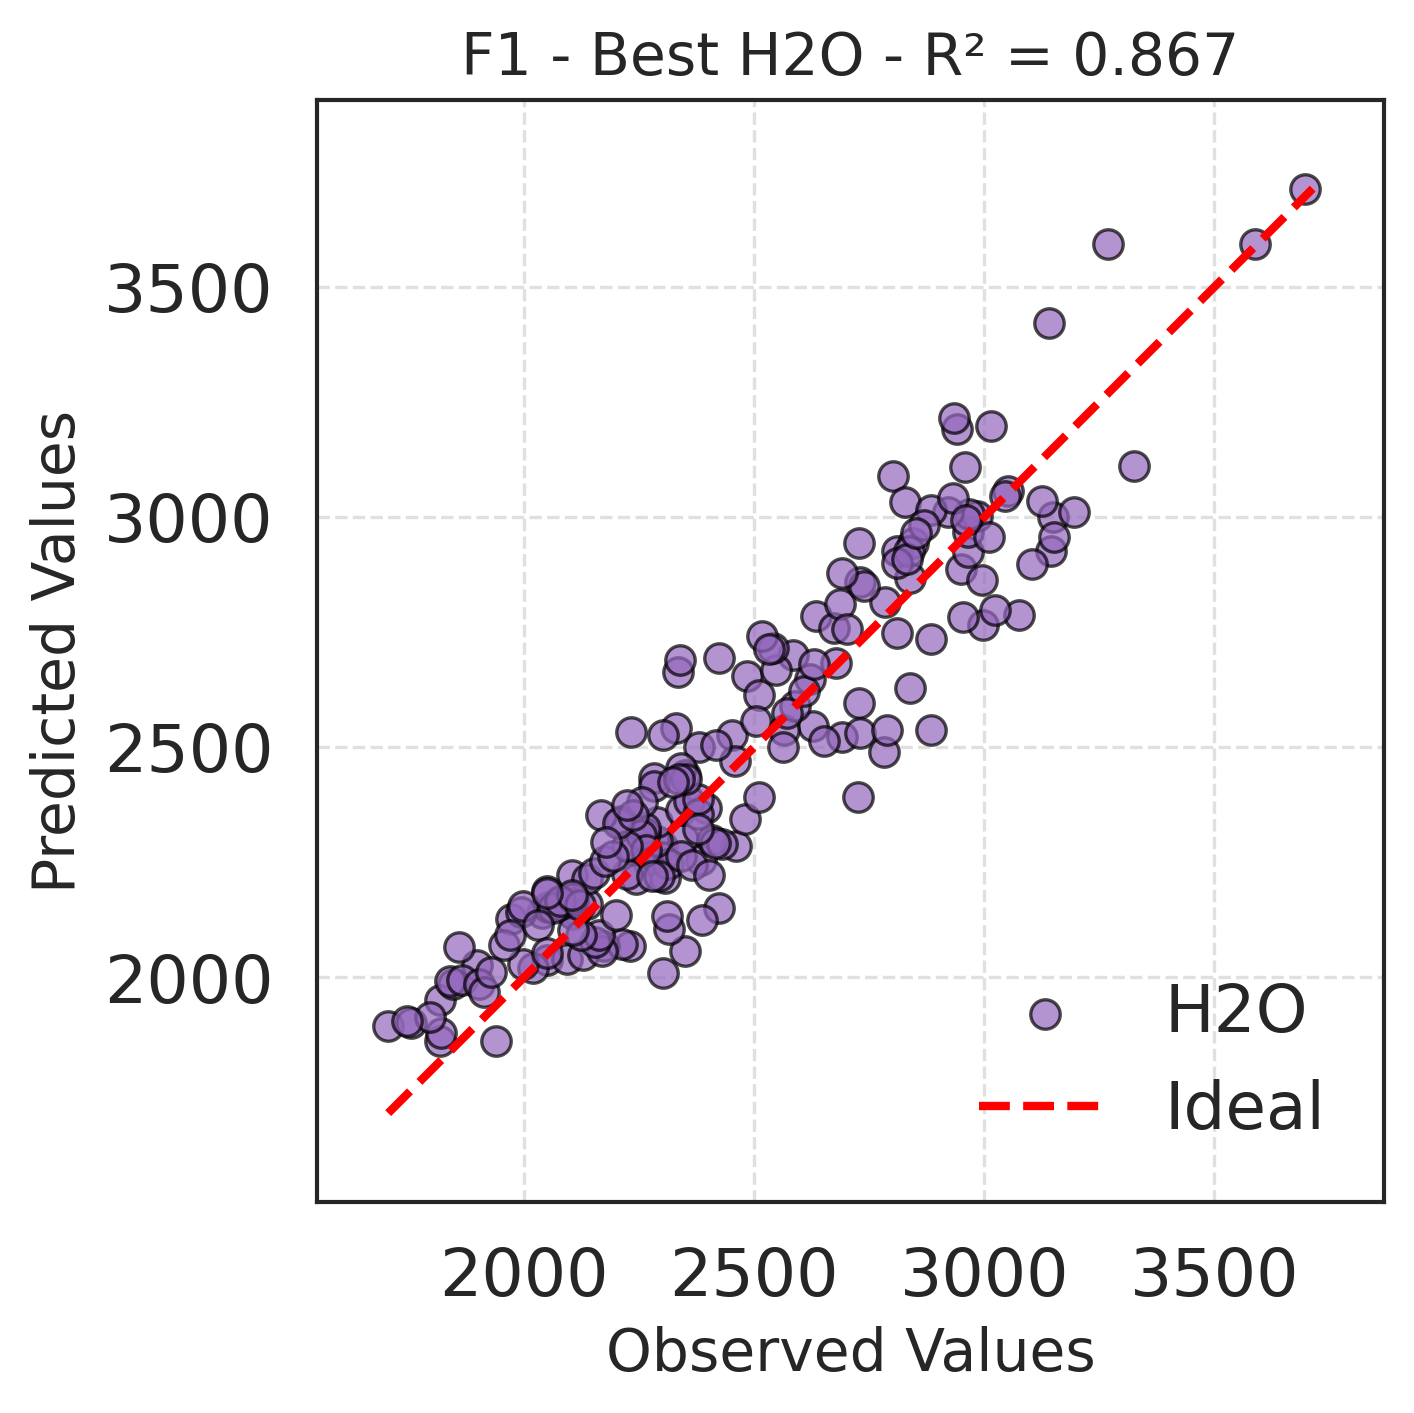
\includegraphics[width=0.8\textwidth]{./img/H2O_best_scatter_F1.png}
    \caption{H2O Best Scatter F1}
    \label{fig:h2o-best-scatter-f1}
\end{figure}

\begin{figure}[htbp]
    \centering
    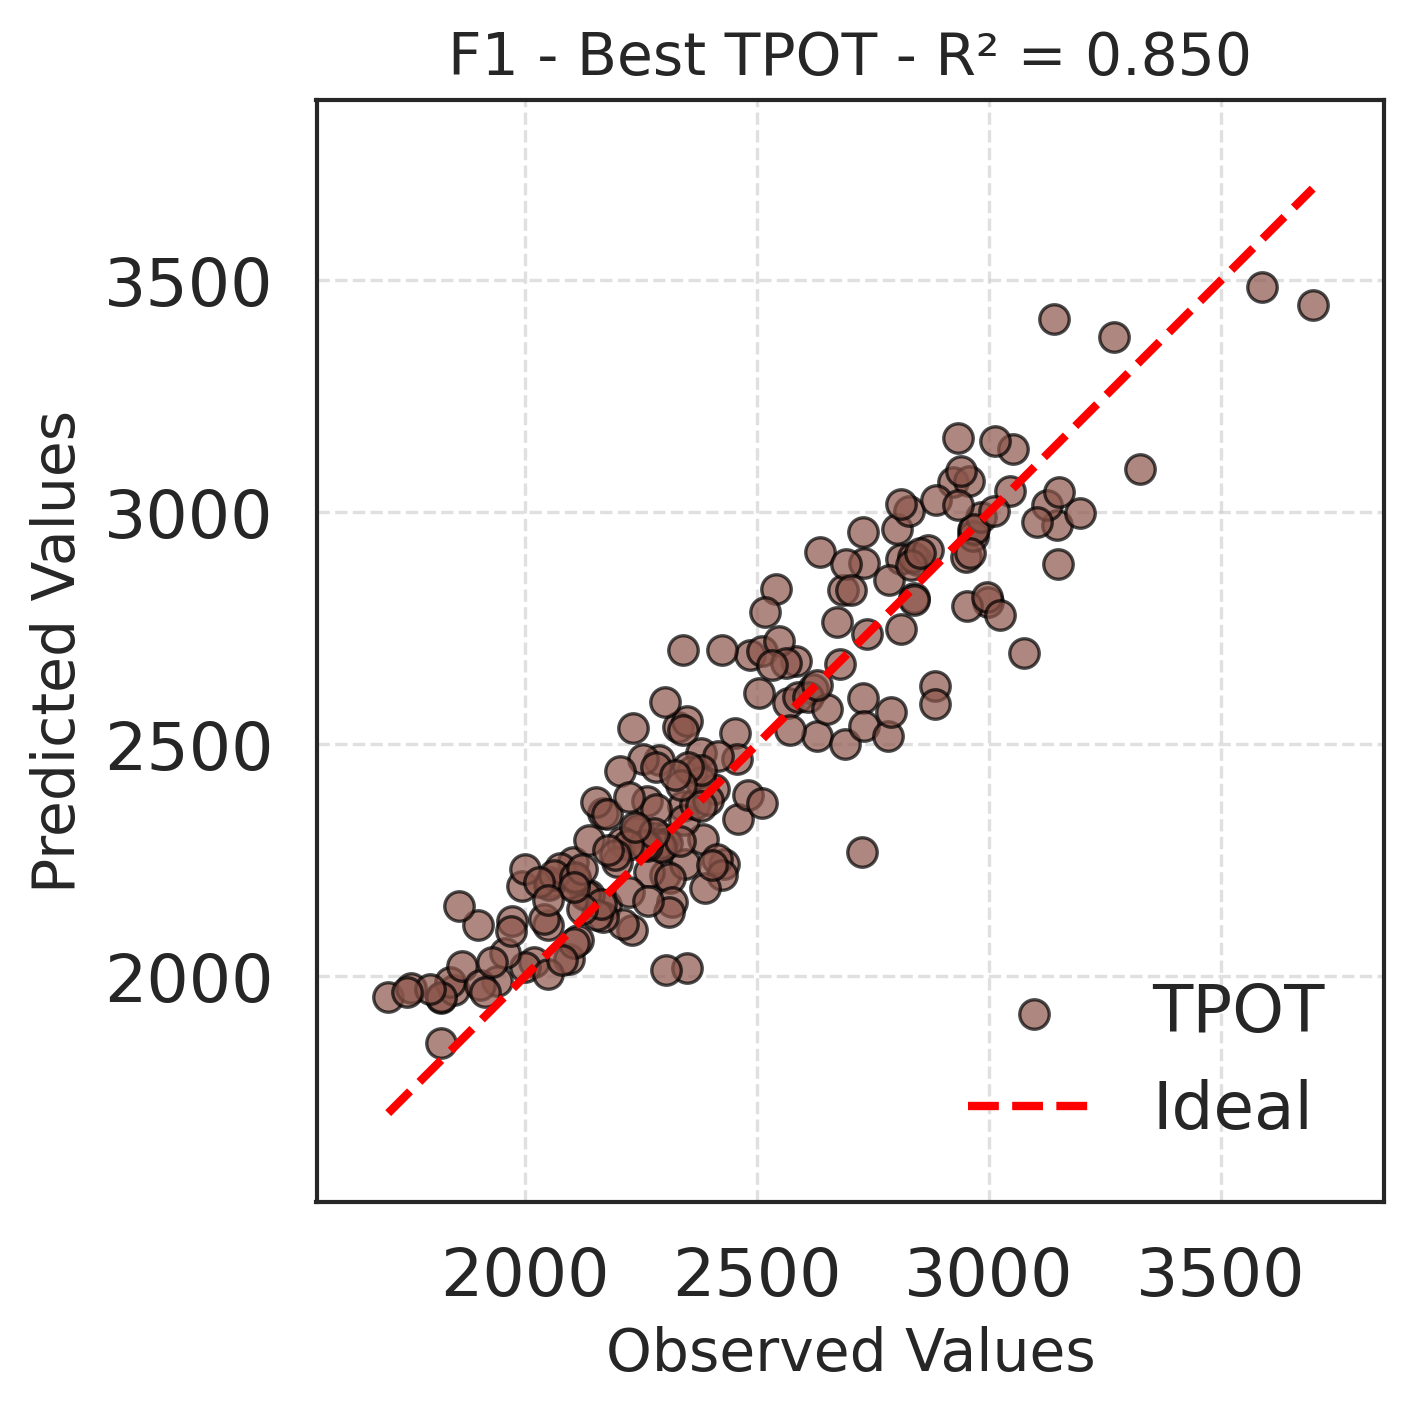
\includegraphics[width=0.8\textwidth]{./img/TPOT_best_scatter_F1.png}
    \caption{Tpot Best Scatter F1}
    \label{fig:tpot-best-scatter-f1}
\end{figure}

\begin{figure}[htbp]
    \centering
    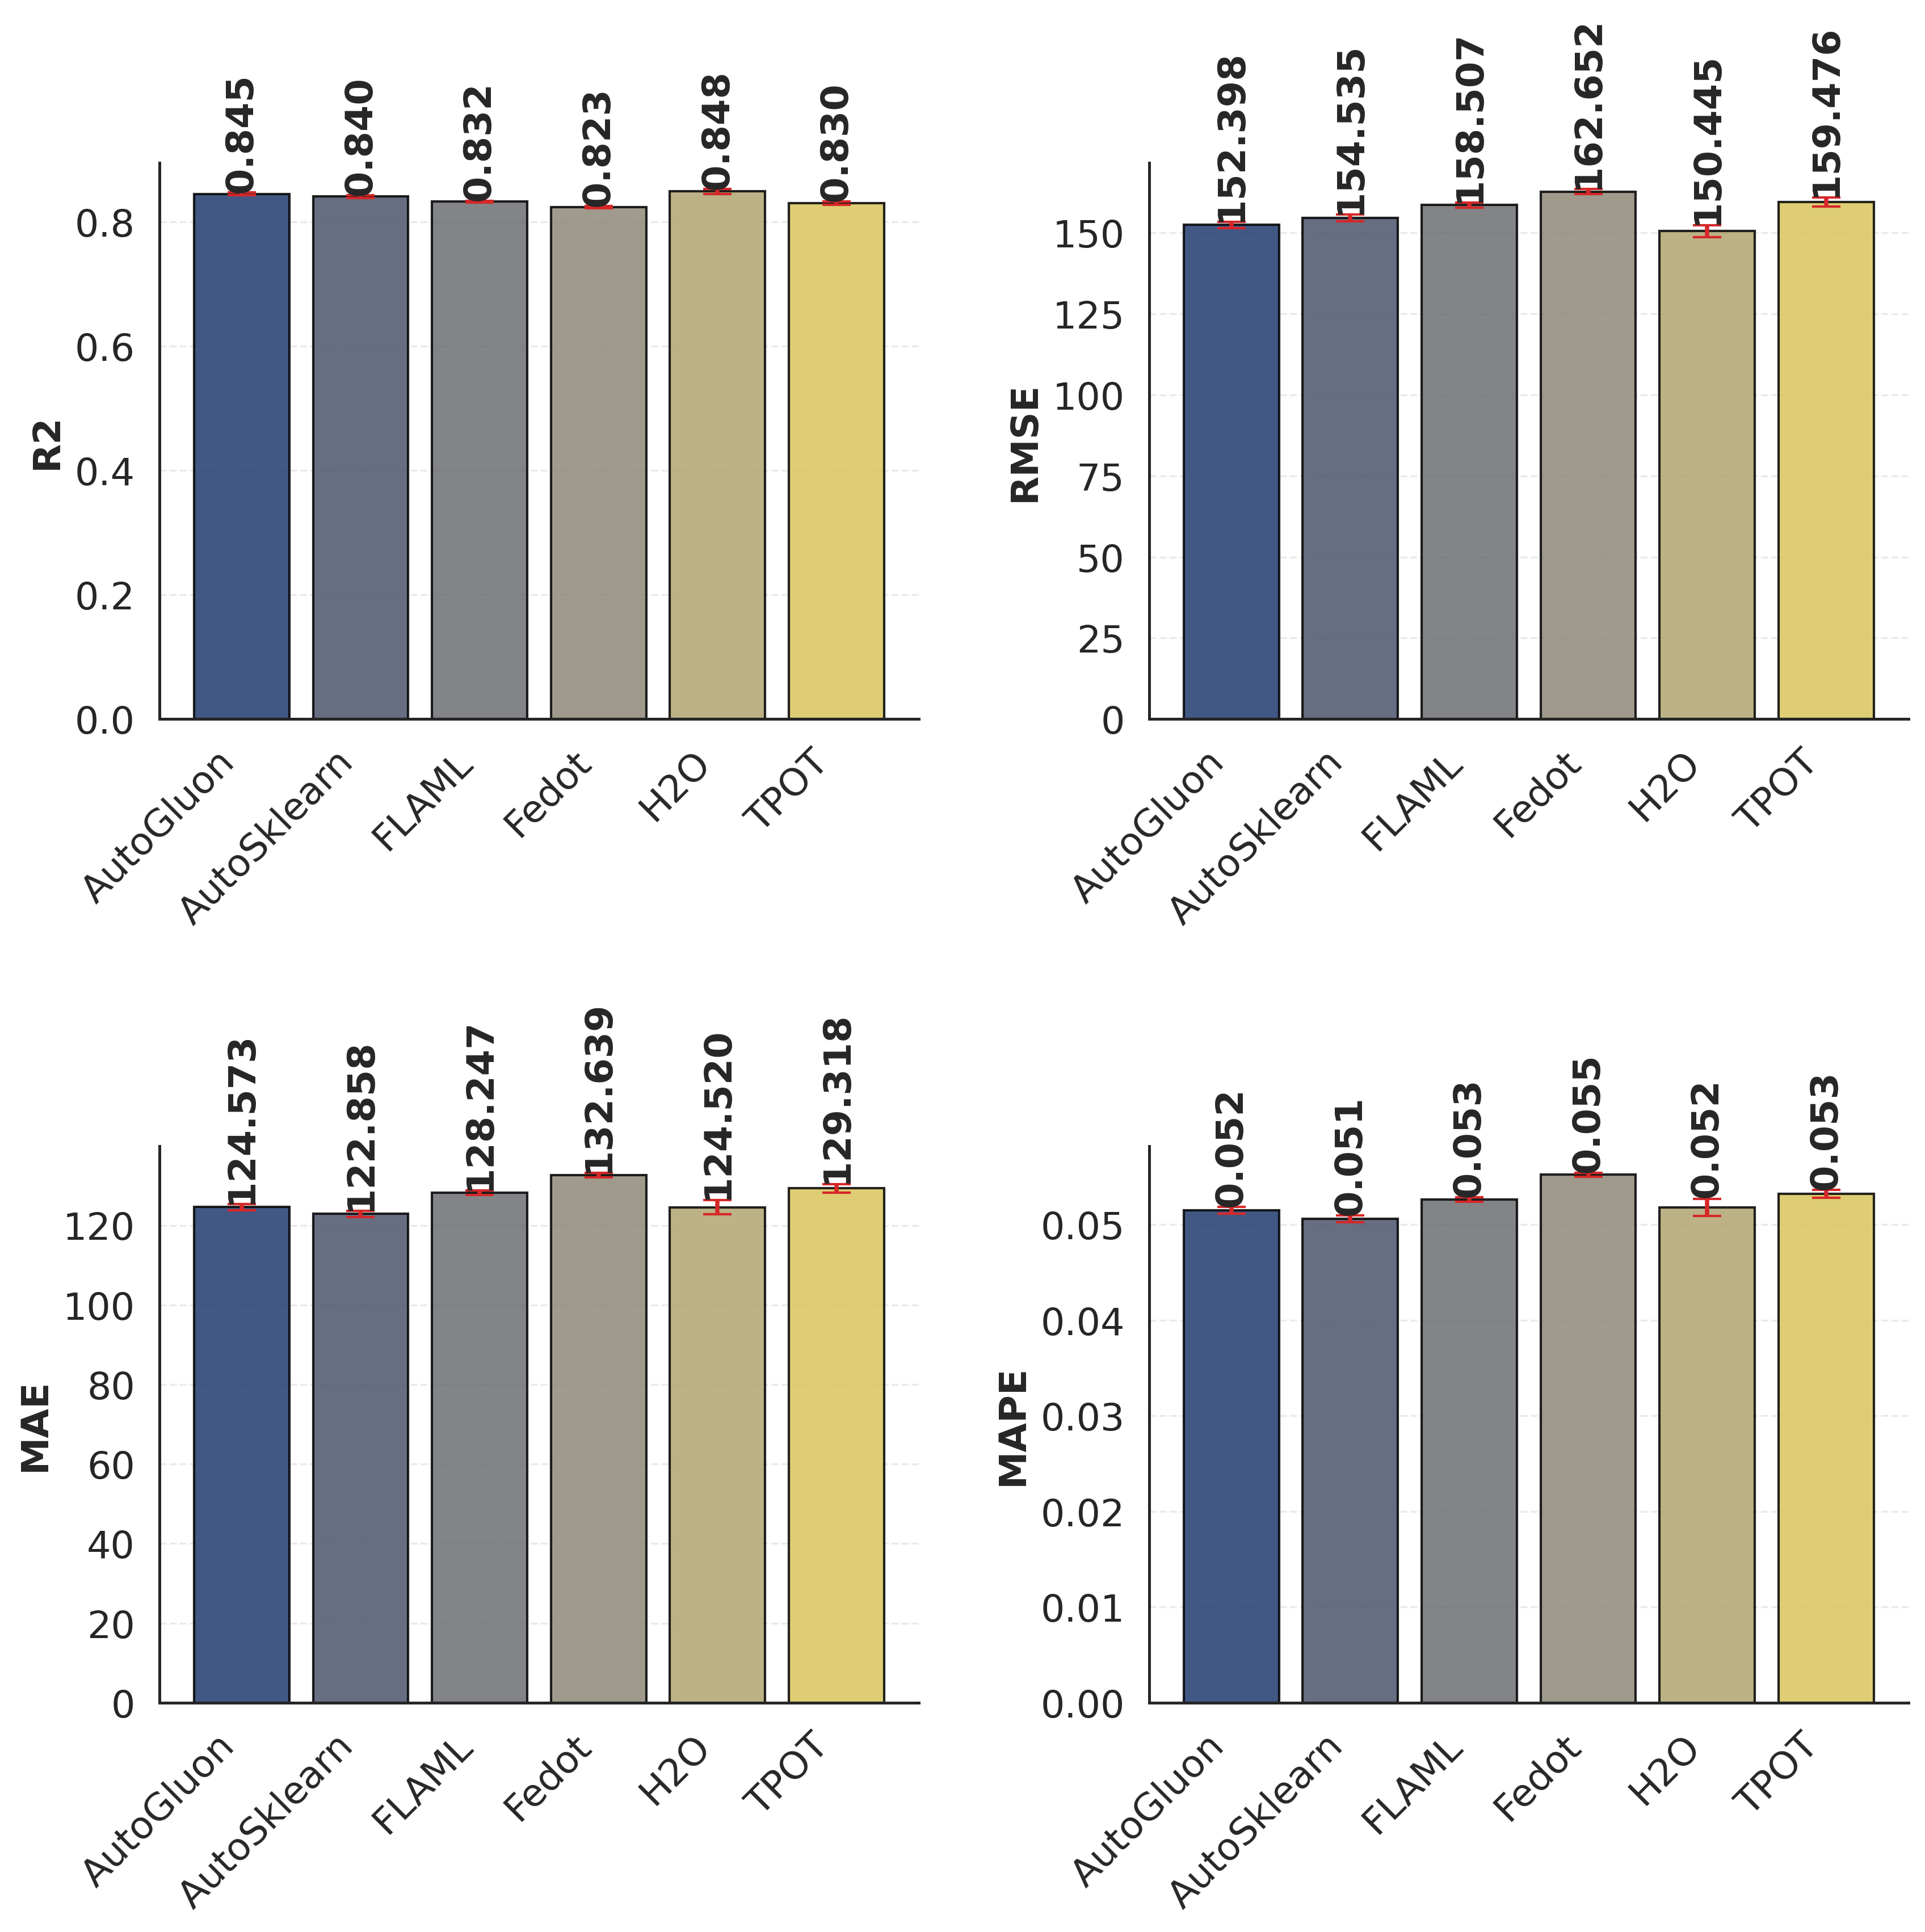
\includegraphics[width=0.8\textwidth]{./img/f1__cmp_metrics.png}
    \caption{F1  Cmp Metrics}
    \label{fig:f1--cmp-metrics}
\end{figure}

\begin{figure}[htbp]
    \centering
    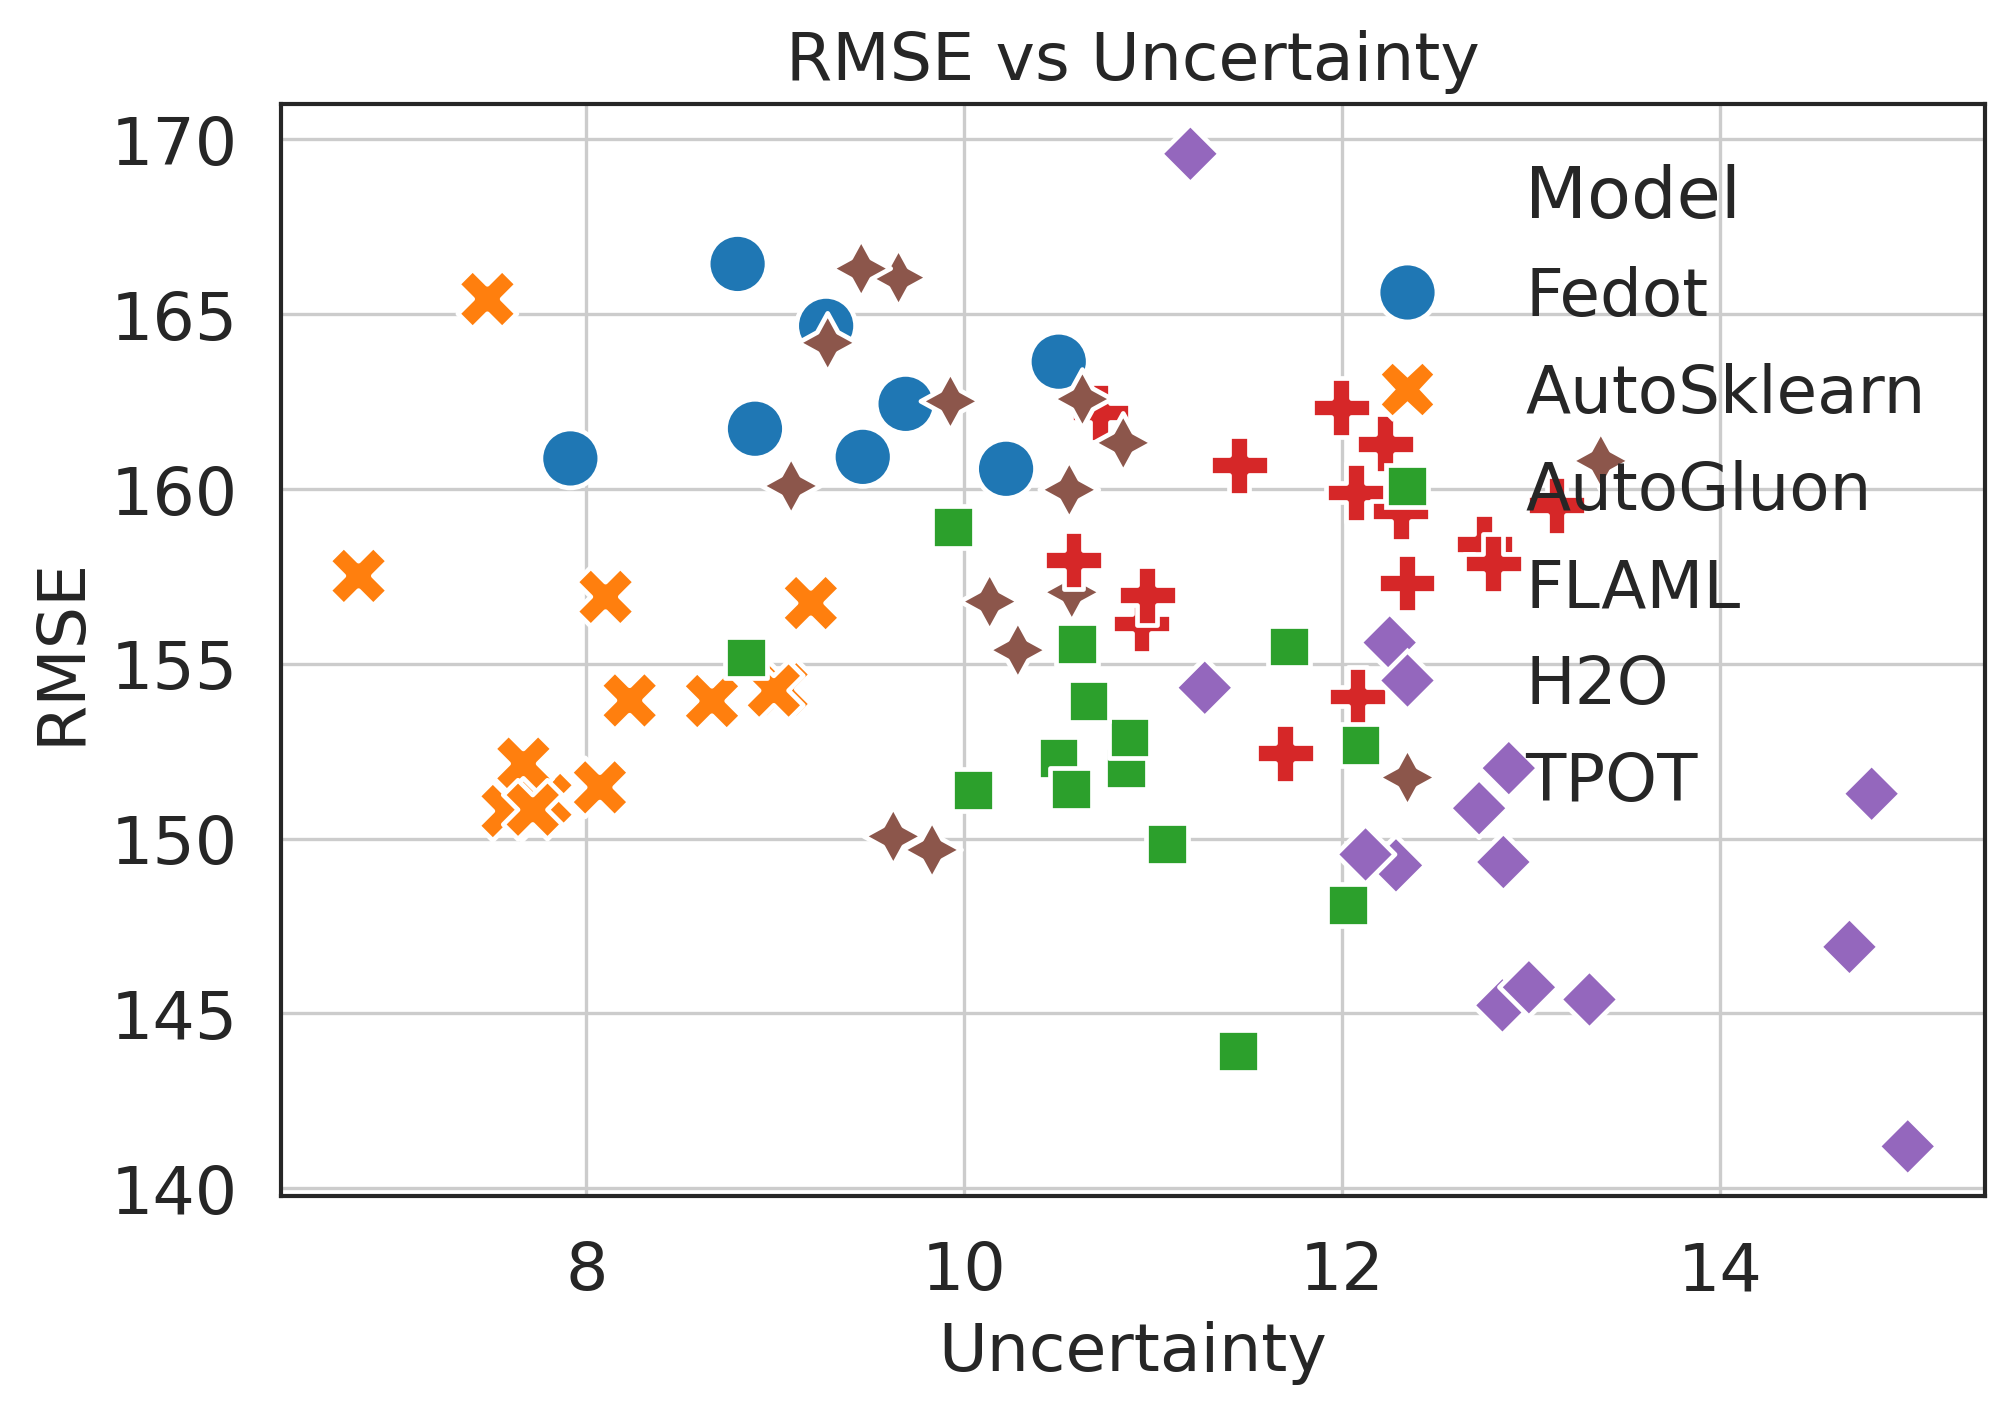
\includegraphics[width=0.8\textwidth]{./img/f1__cmp_uncertainty.png}
    \caption{F1  Cmp Uncertainty}
    \label{fig:f1--cmp-uncertainty}
\end{figure}

\begin{figure}[htbp]
    \centering
    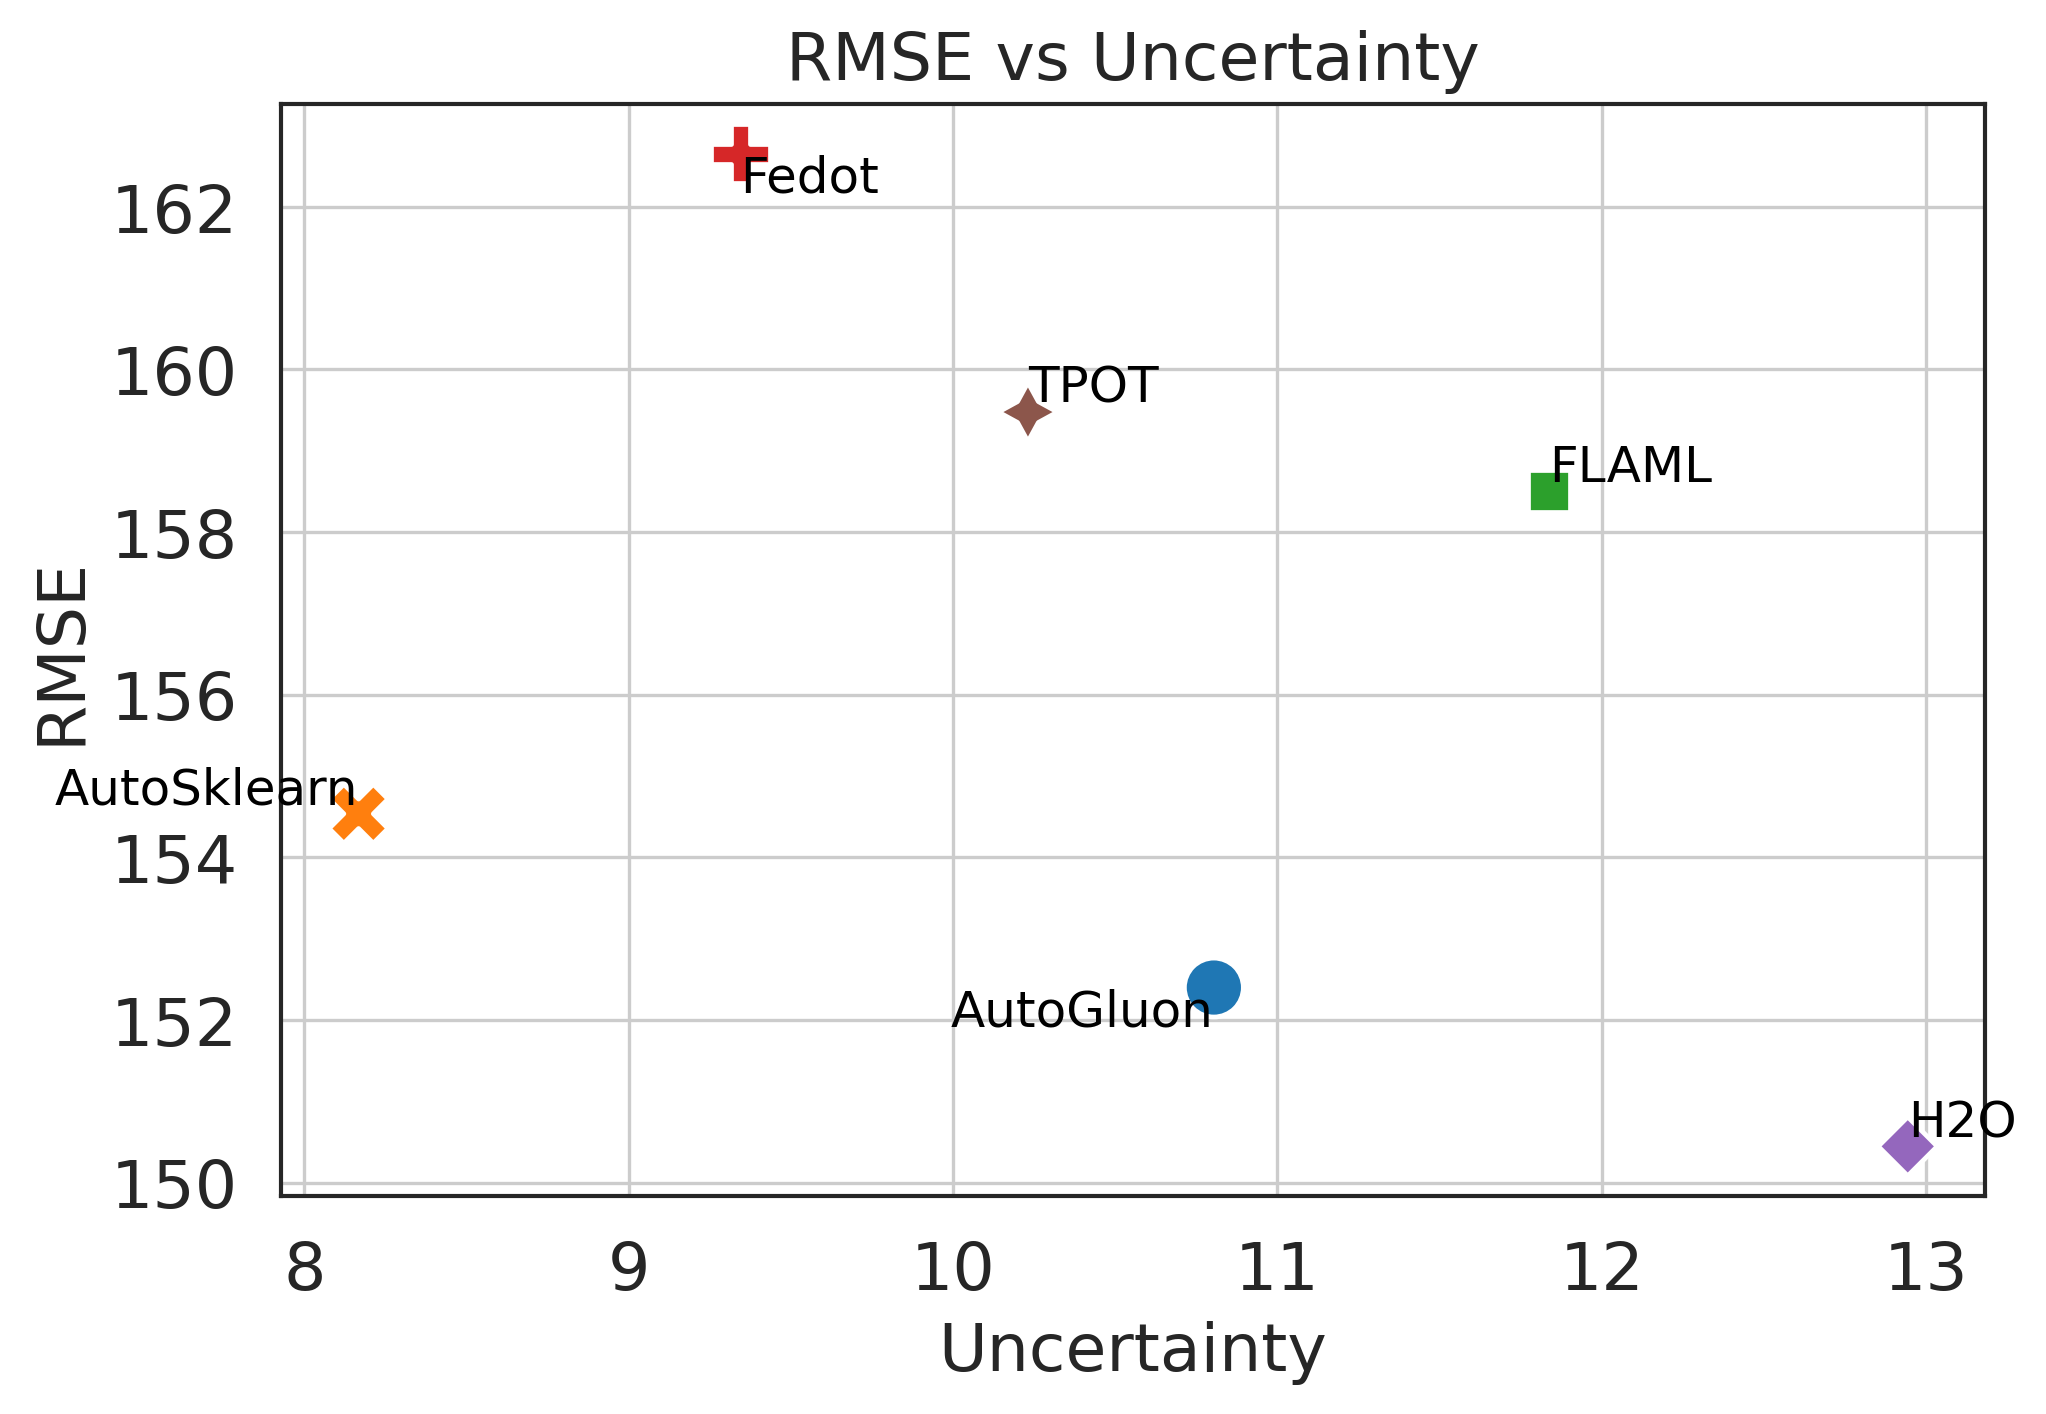
\includegraphics[width=0.8\textwidth]{./img/f1__cmp_uncertainty_grouped.png}
    \caption{F1  Cmp Uncertainty Grouped}
    \label{fig:f1--cmp-uncertainty-grouped}
\end{figure}

\begin{figure}[htbp]
    \centering
    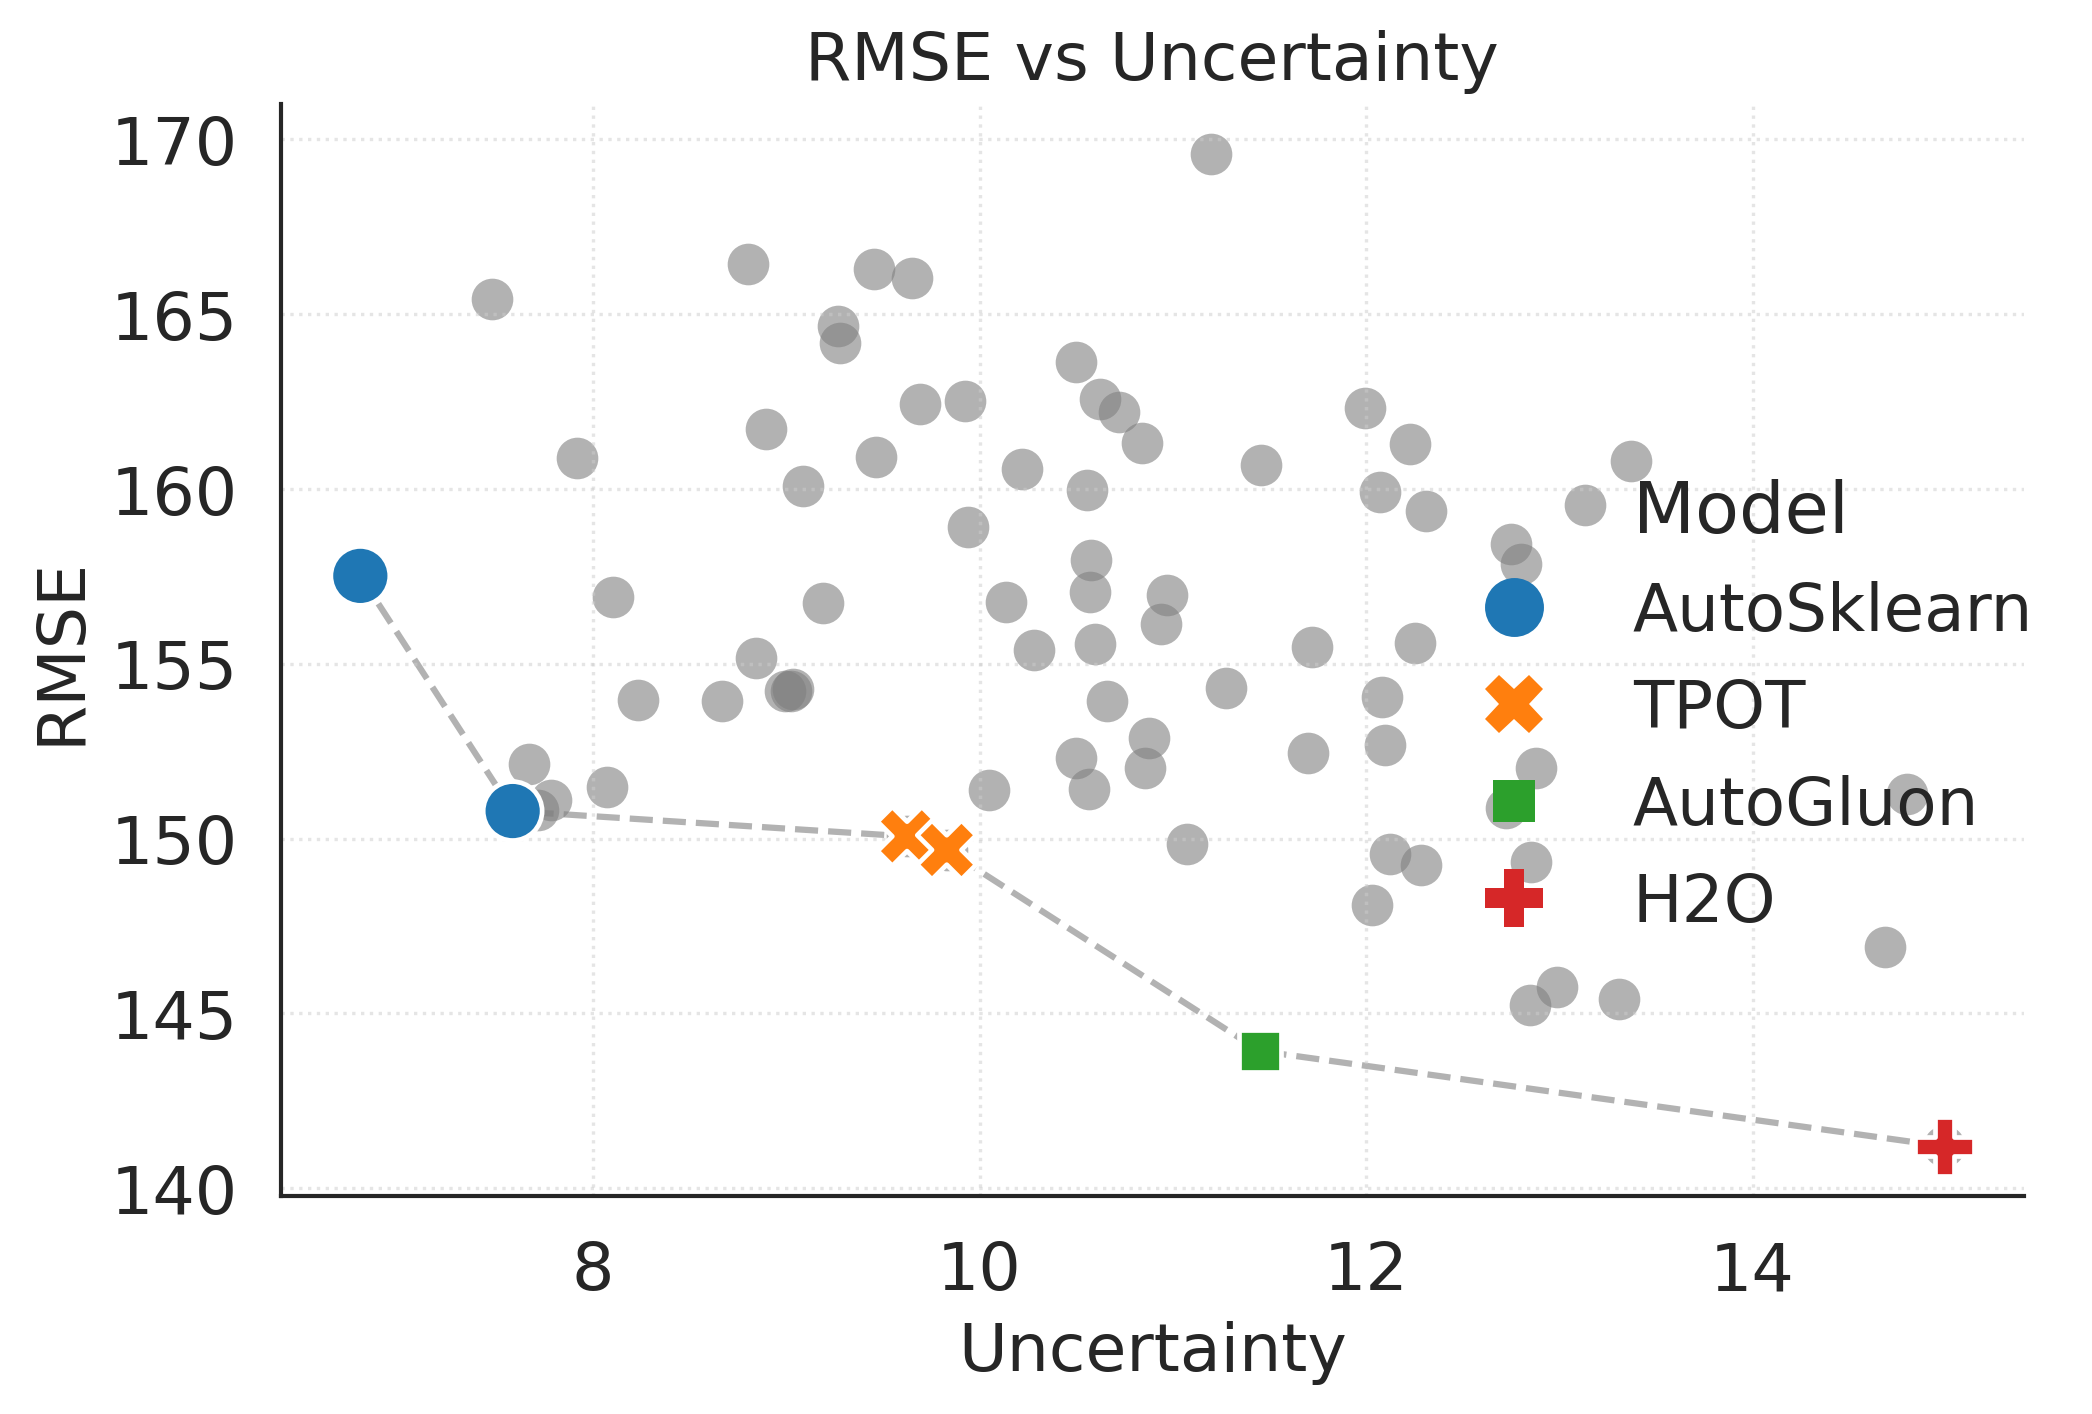
\includegraphics[width=0.8\textwidth]{./img/f1__cmp_uncertainty_pareto.png}
    \caption{F1  Cmp Uncertainty Pareto}
    \label{fig:f1--cmp-uncertainty-pareto}
\end{figure}

\begin{figure}[htbp]
    \centering
    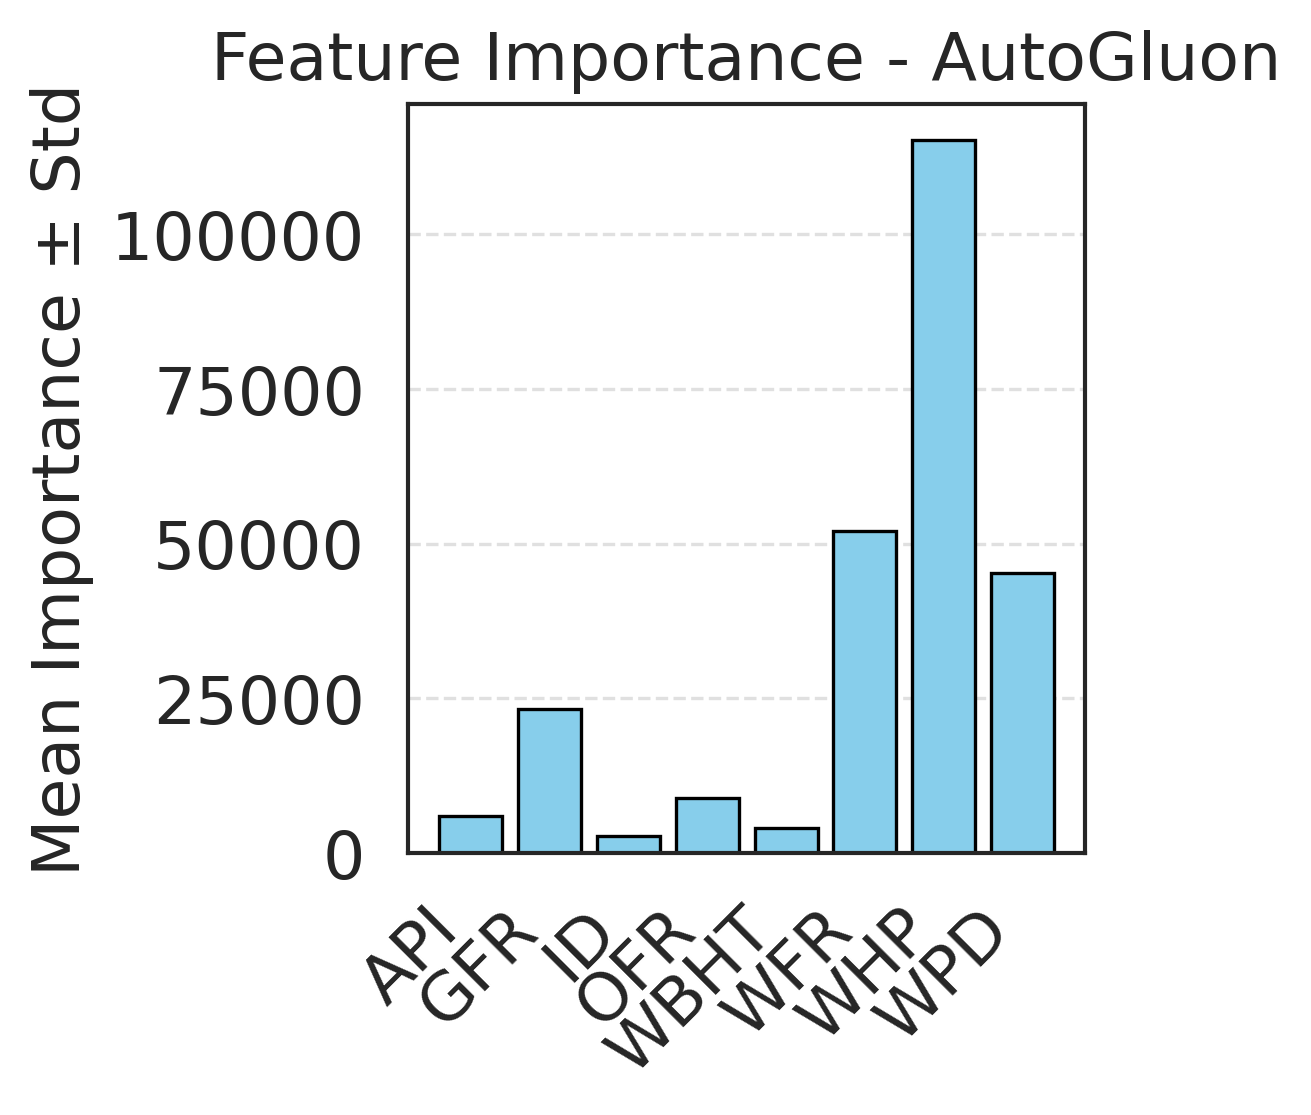
\includegraphics[width=0.8\textwidth]{./img/f1__fi_AutoGluon.png}
    \caption{F1  Fi Autogluon}
    \label{fig:f1--fi-autogluon}
\end{figure}

\begin{figure}[htbp]
    \centering
    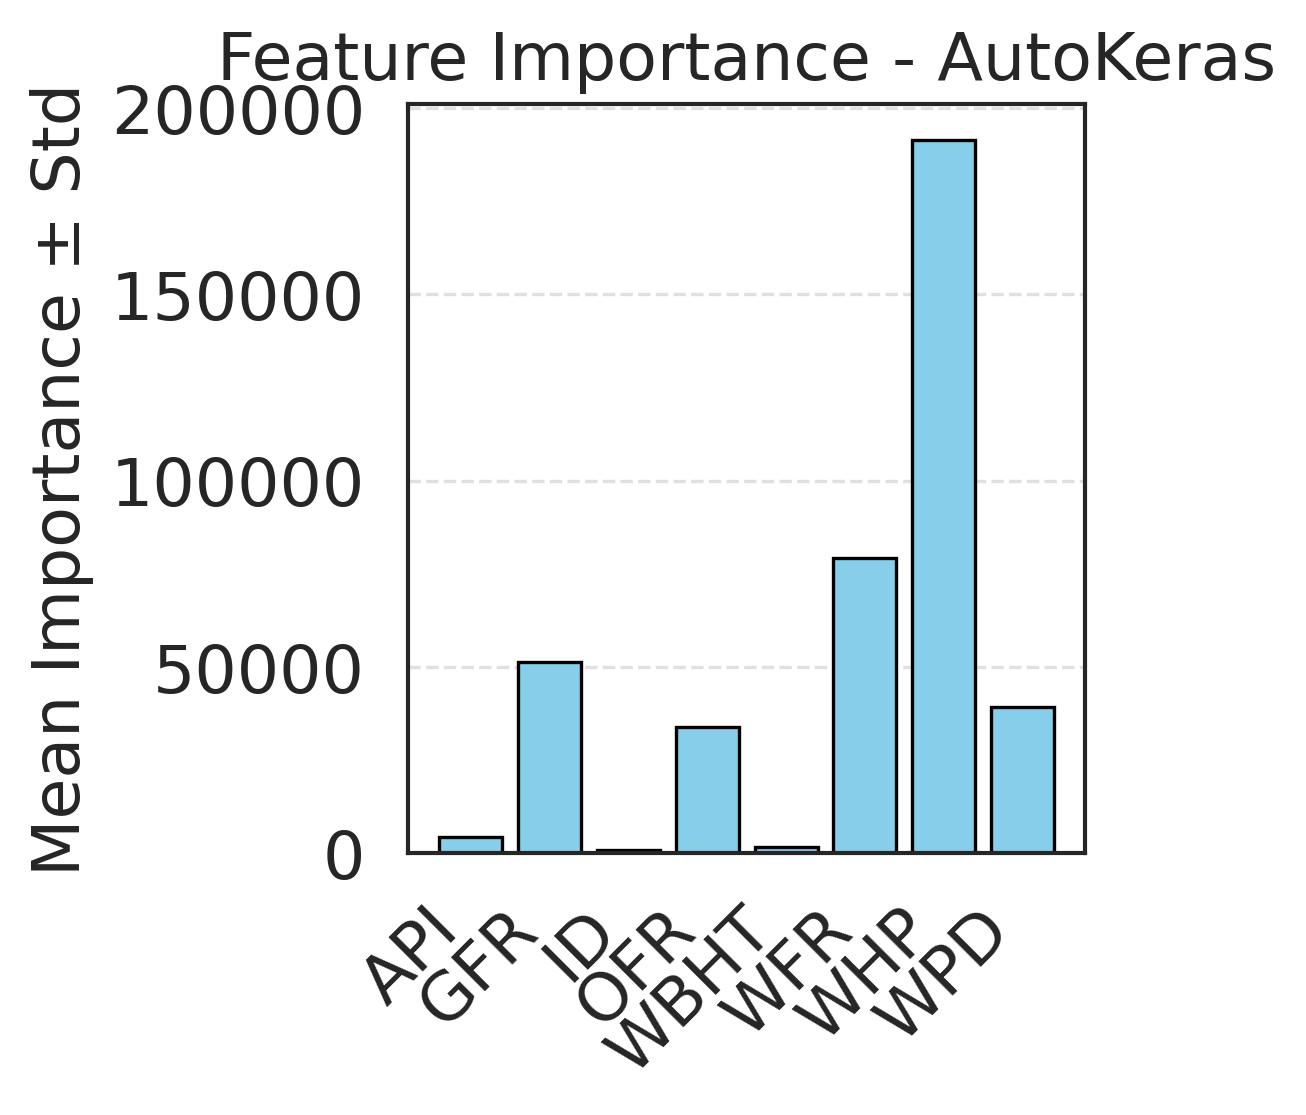
\includegraphics[width=0.8\textwidth]{./img/f1__fi_AutoKeras.png}
    \caption{F1  Fi Autokeras}
    \label{fig:f1--fi-autokeras}
\end{figure}

\begin{figure}[htbp]
    \centering
    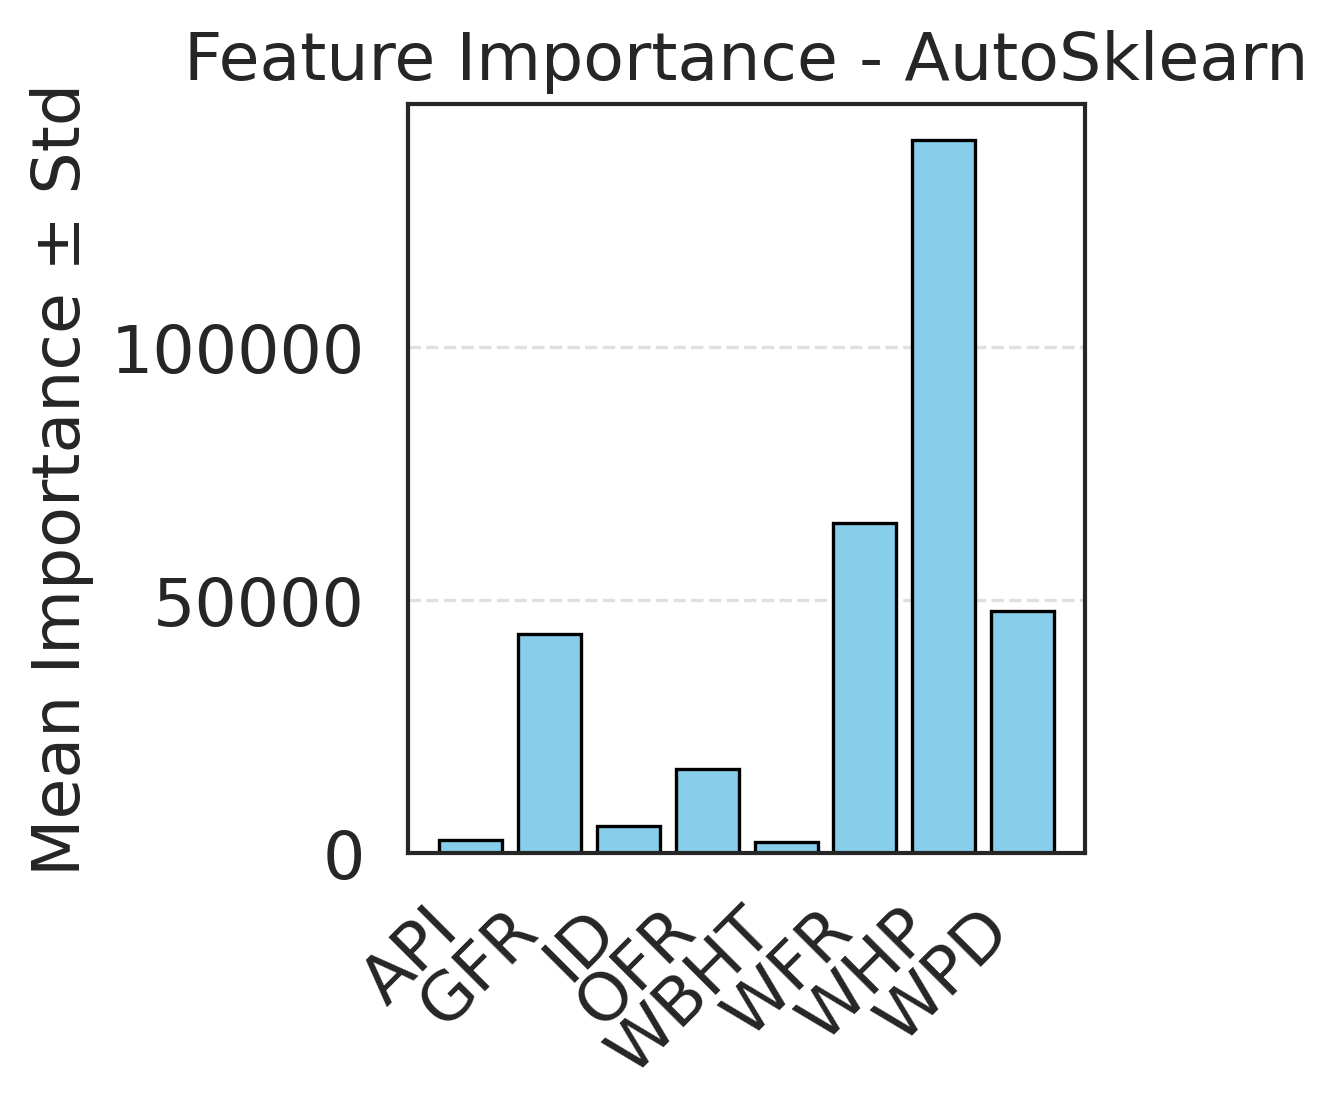
\includegraphics[width=0.8\textwidth]{./img/f1__fi_AutoSklearn.png}
    \caption{F1  Fi Autosklearn}
    \label{fig:f1--fi-autosklearn}
\end{figure}

\begin{figure}[htbp]
    \centering
    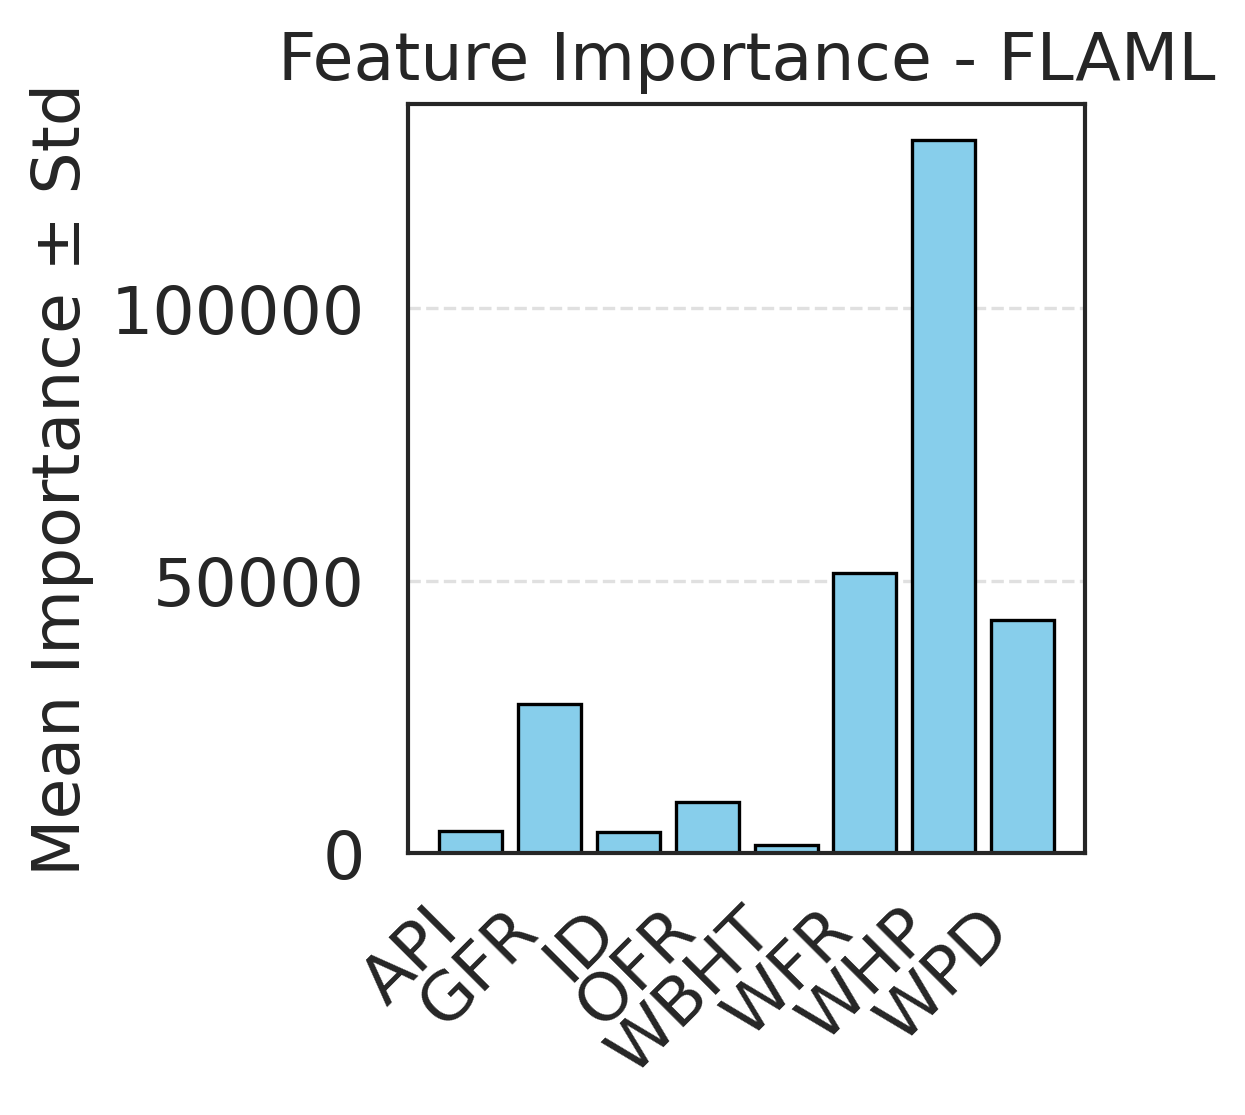
\includegraphics[width=0.8\textwidth]{./img/f1__fi_FLAML.png}
    \caption{F1  Fi Flaml}
    \label{fig:f1--fi-flaml}
\end{figure}

\begin{figure}[htbp]
    \centering
    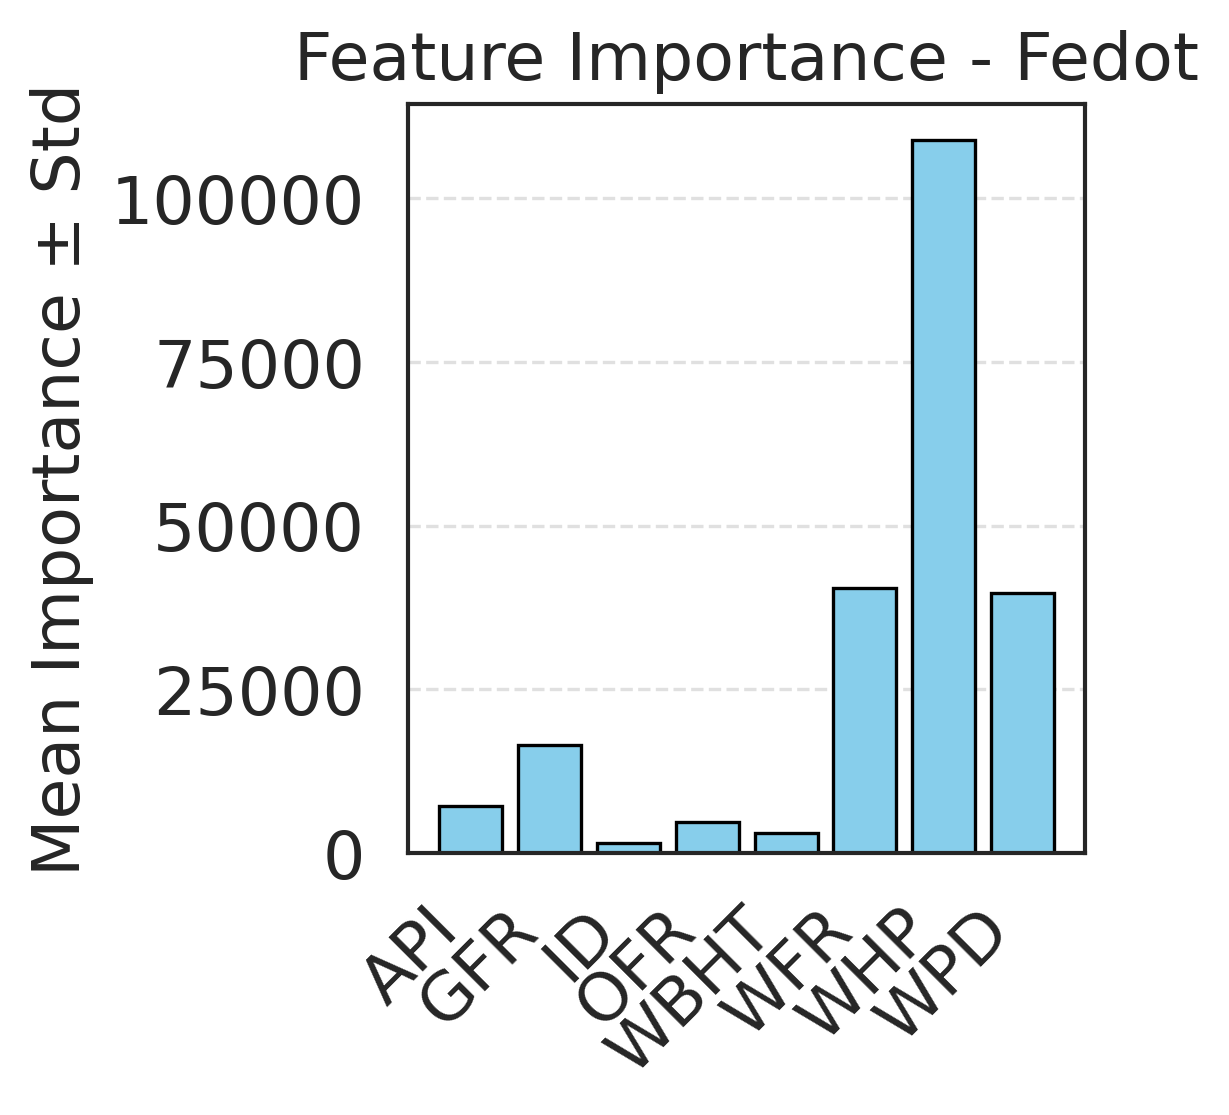
\includegraphics[width=0.8\textwidth]{./img/f1__fi_Fedot.png}
    \caption{F1  Fi Fedot}
    \label{fig:f1--fi-fedot}
\end{figure}

\begin{figure}[htbp]
    \centering
    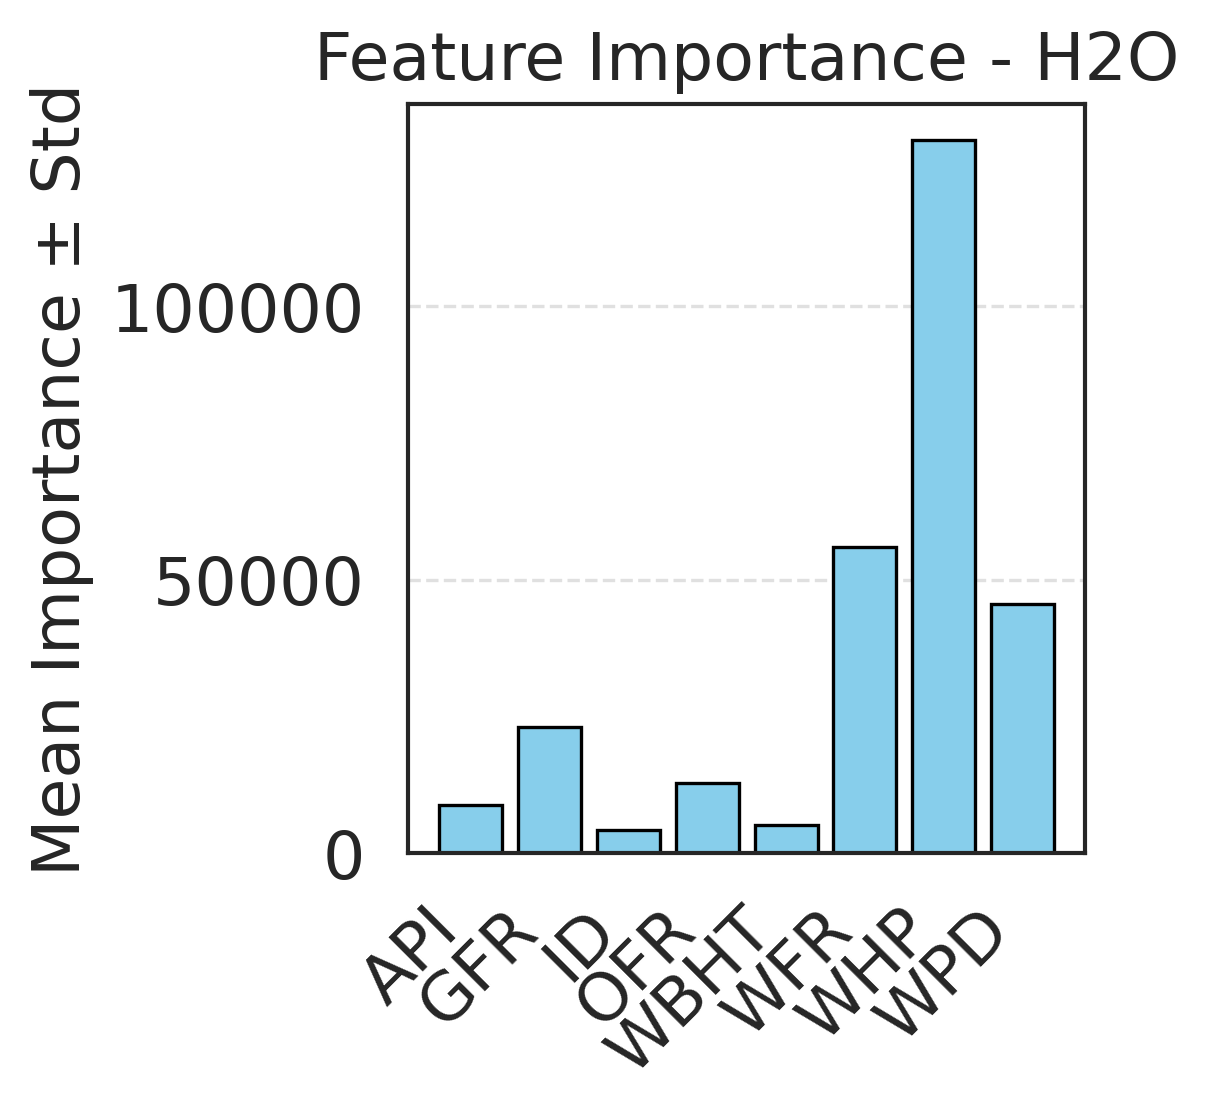
\includegraphics[width=0.8\textwidth]{./img/f1__fi_H2O.png}
    \caption{F1  Fi H2O}
    \label{fig:f1--fi-h2o}
\end{figure}

\begin{figure}[htbp]
    \centering
    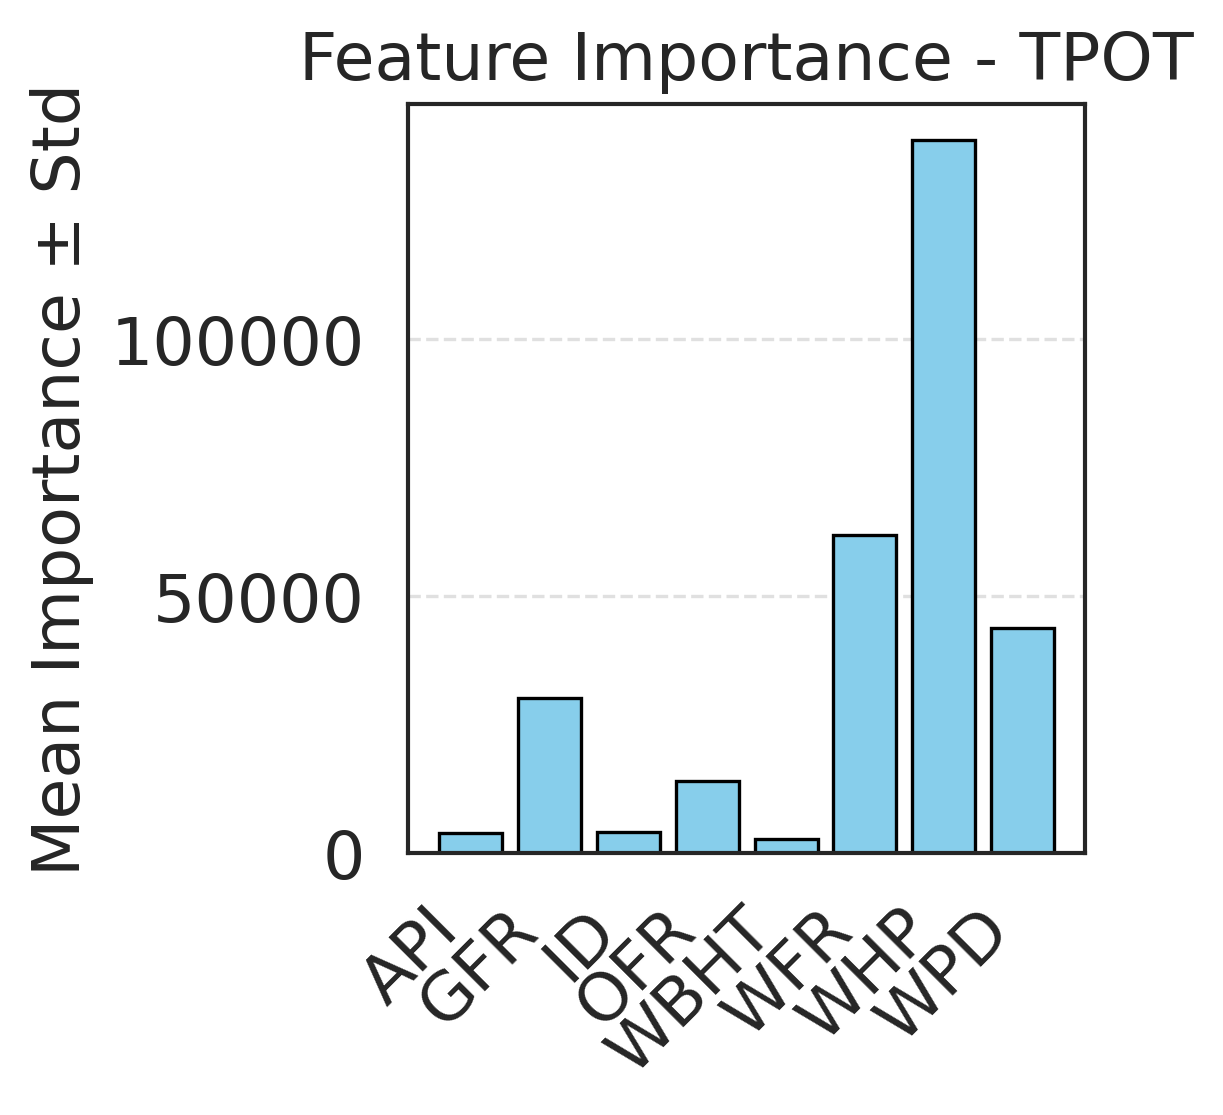
\includegraphics[width=0.8\textwidth]{./img/f1__fi_TPOT.png}
    \caption{F1  Fi Tpot}
    \label{fig:f1--fi-tpot}
\end{figure}

\begin{figure}[htbp]
    \centering
    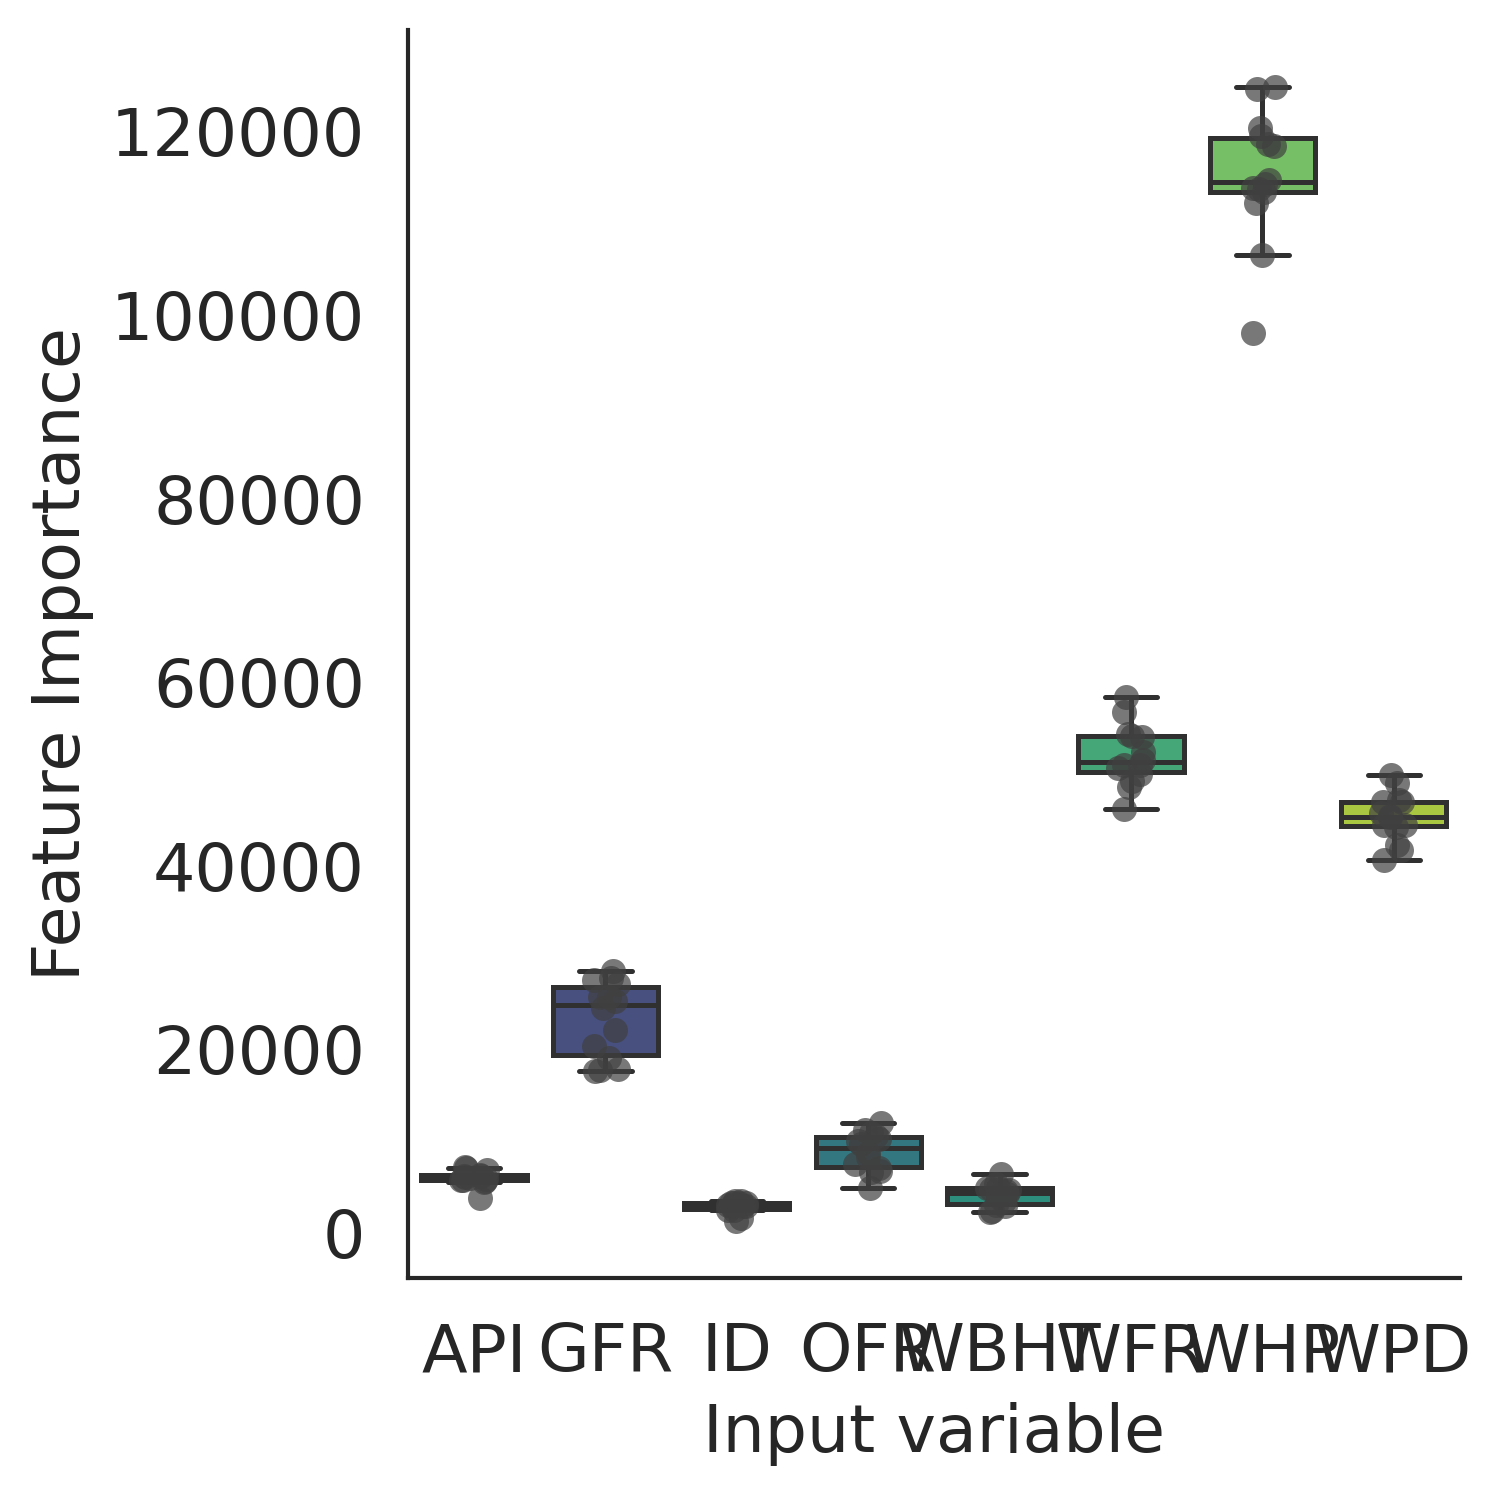
\includegraphics[width=0.8\textwidth]{./img/f1__fi_bxp_AutoGluon.png}
    \caption{F1  Fi Bxp Autogluon}
    \label{fig:f1--fi-bxp-autogluon}
\end{figure}

\begin{figure}[htbp]
    \centering
    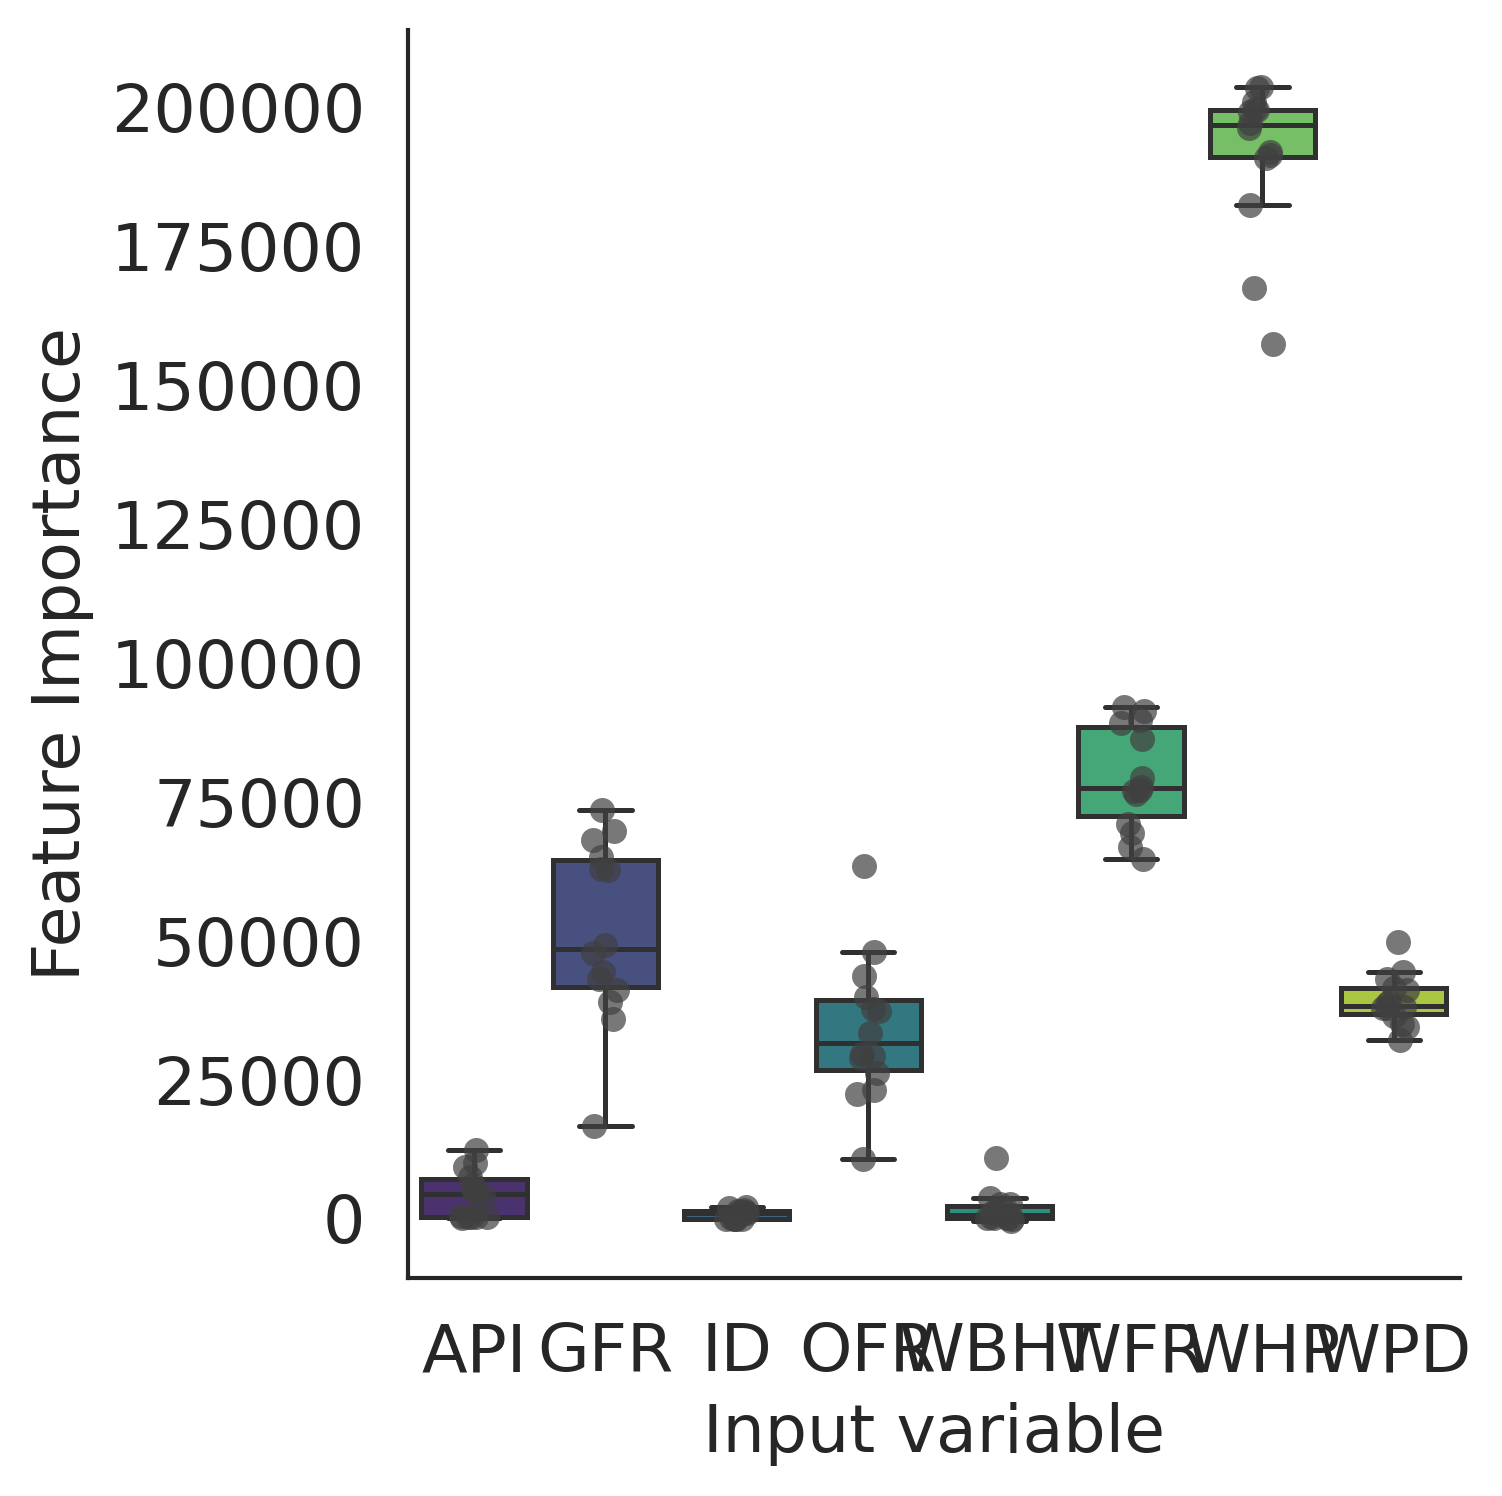
\includegraphics[width=0.8\textwidth]{./img/f1__fi_bxp_AutoKeras.png}
    \caption{F1  Fi Bxp Autokeras}
    \label{fig:f1--fi-bxp-autokeras}
\end{figure}

\begin{figure}[htbp]
    \centering
    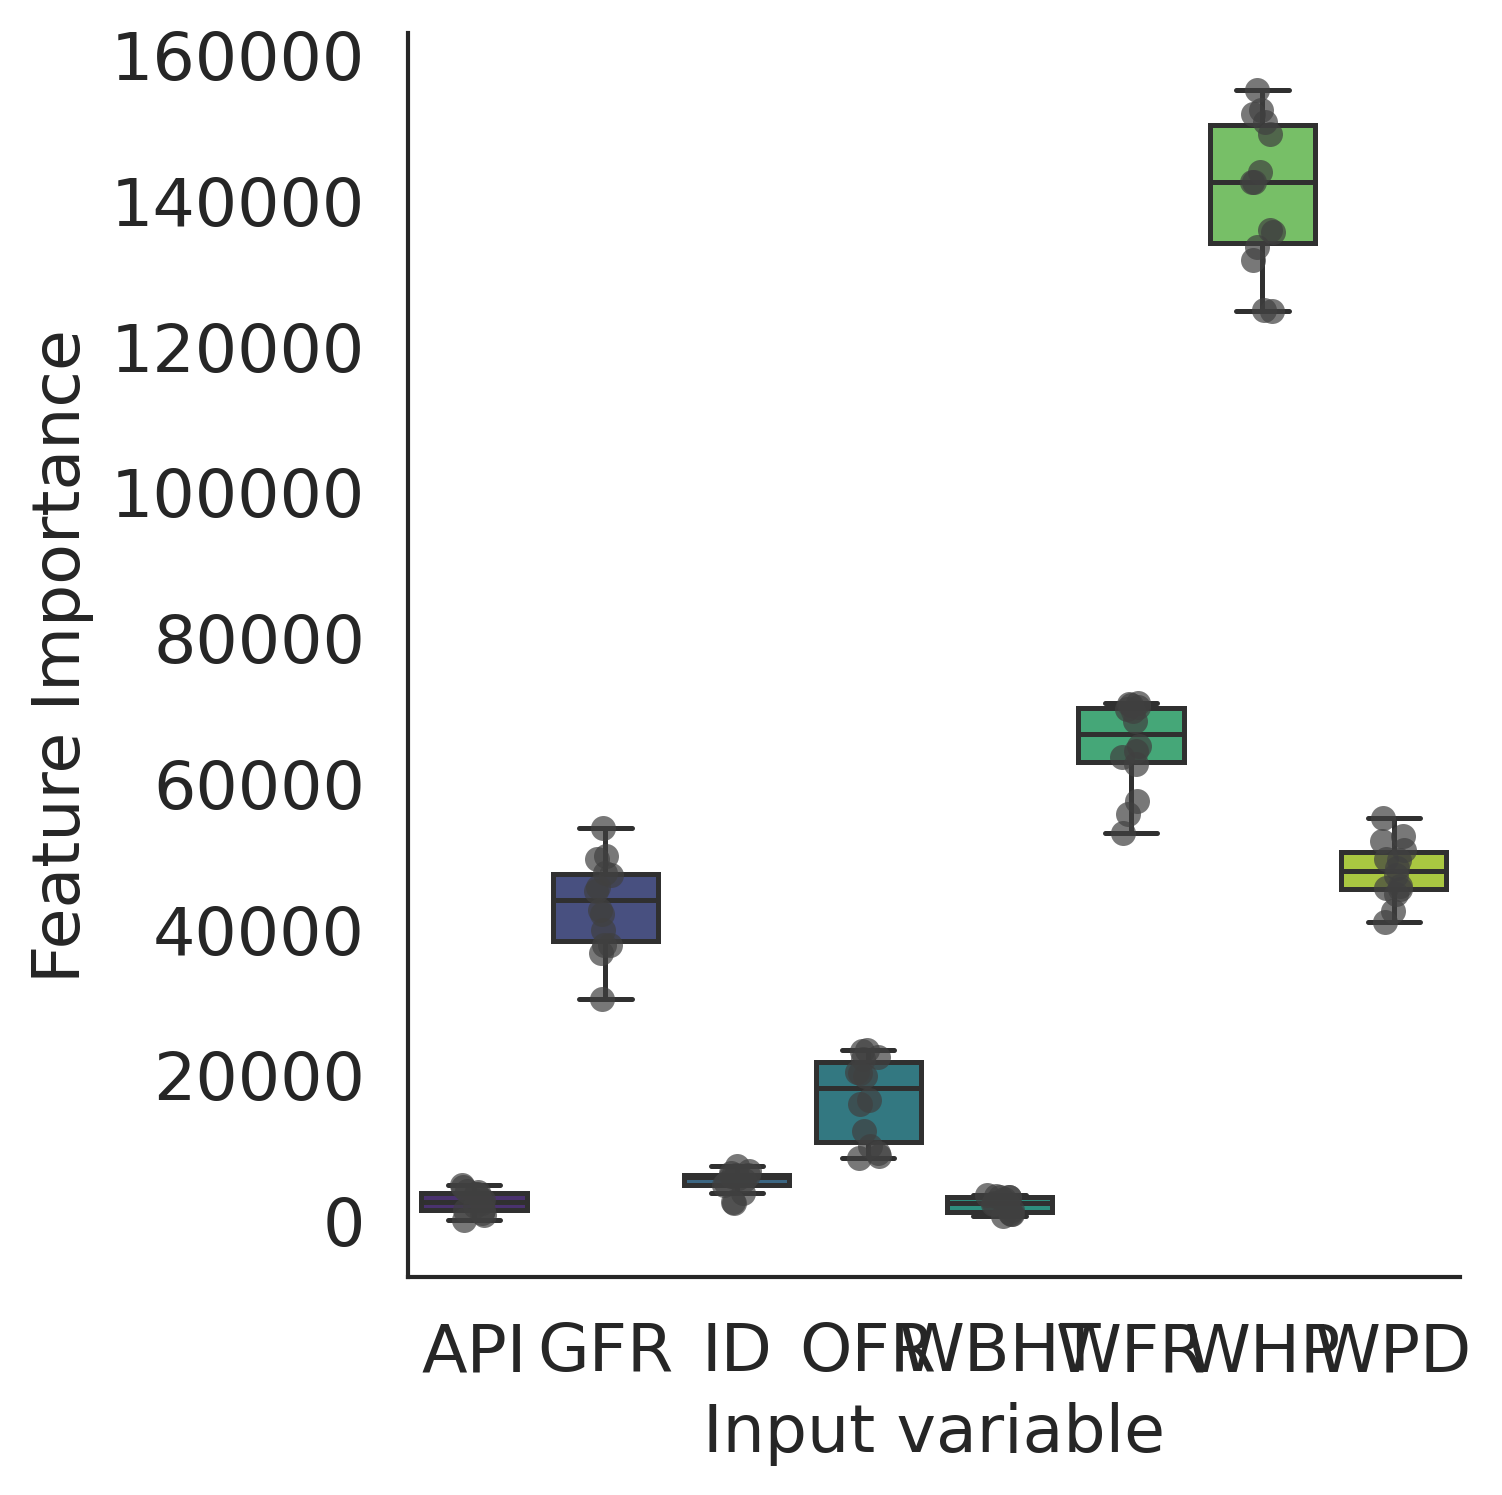
\includegraphics[width=0.8\textwidth]{./img/f1__fi_bxp_AutoSklearn.png}
    \caption{F1  Fi Bxp Autosklearn}
    \label{fig:f1--fi-bxp-autosklearn}
\end{figure}

\begin{figure}[htbp]
    \centering
    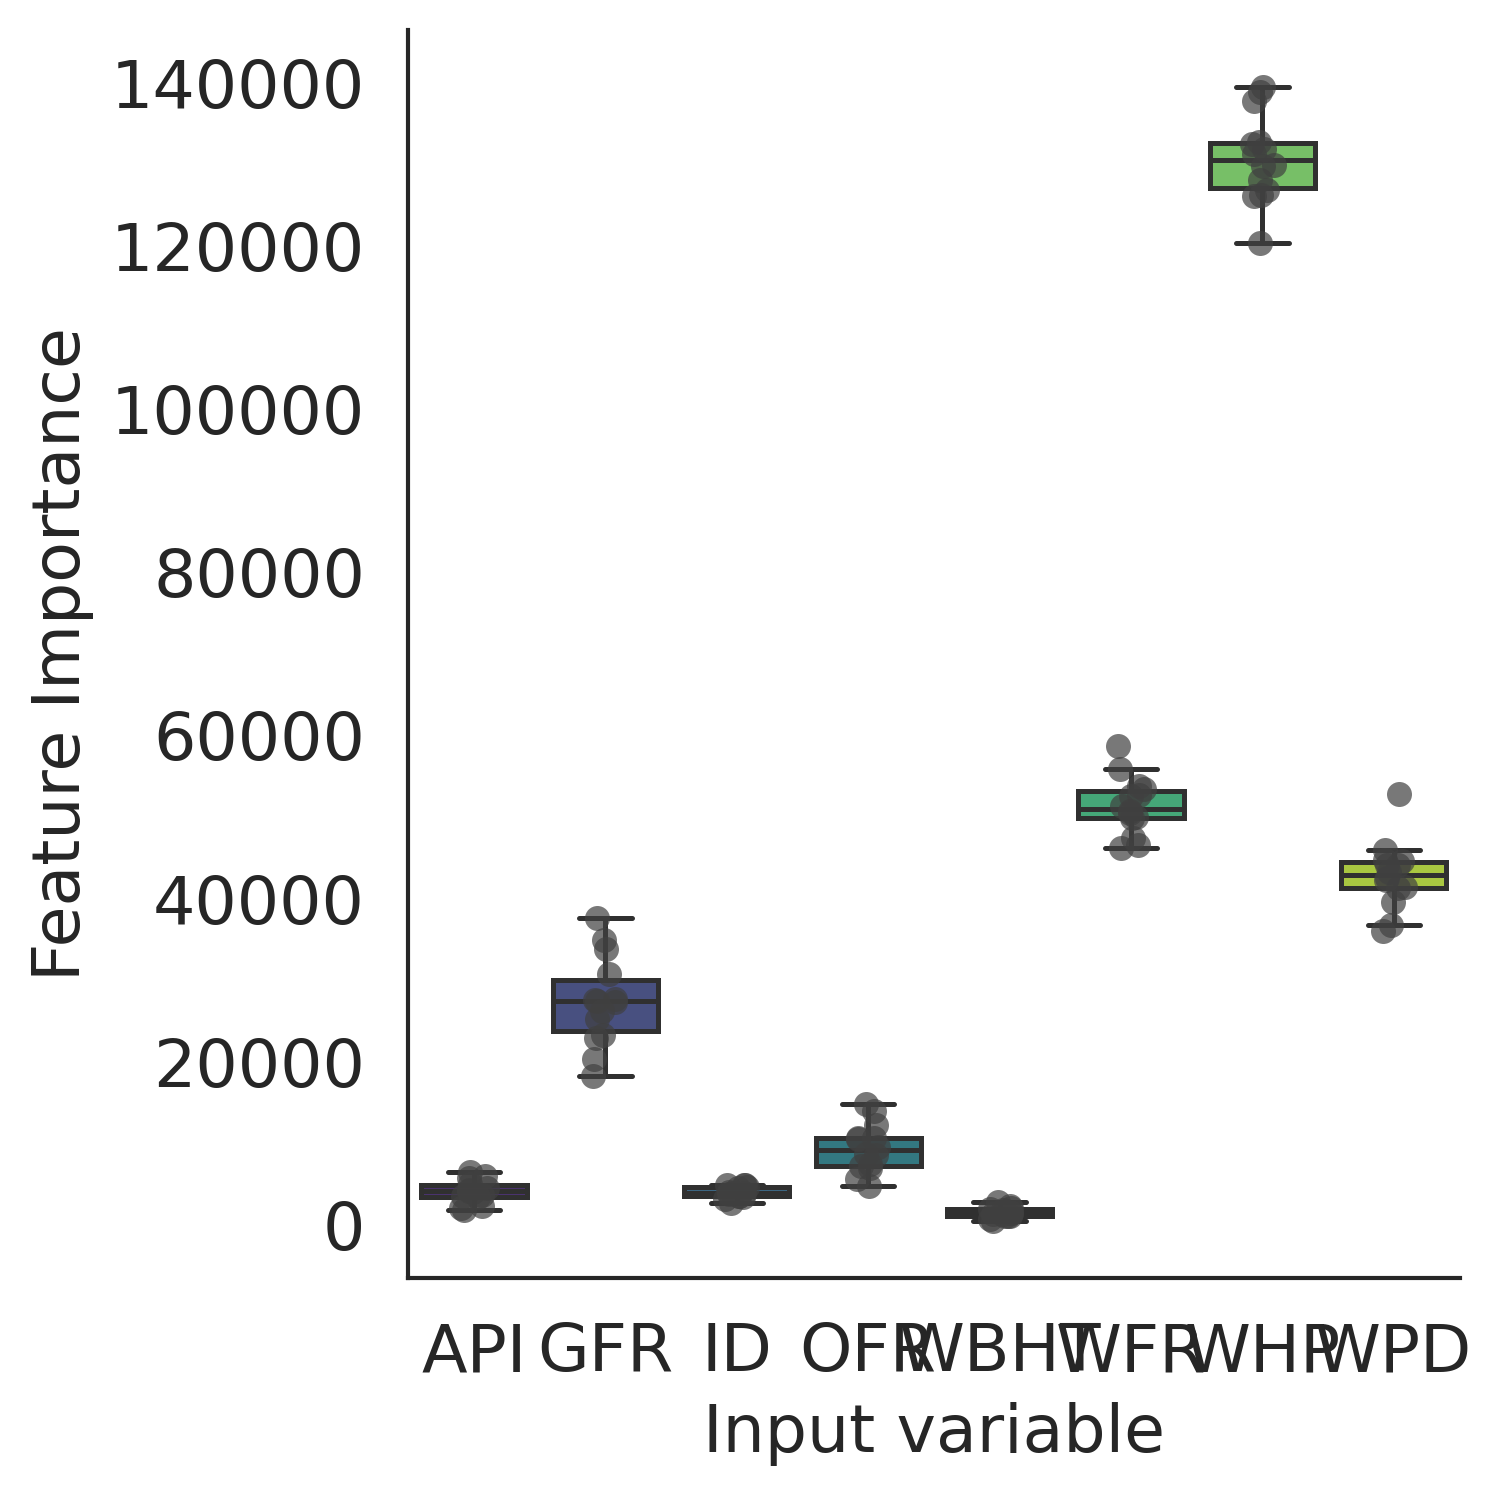
\includegraphics[width=0.8\textwidth]{./img/f1__fi_bxp_FLAML.png}
    \caption{F1  Fi Bxp Flaml}
    \label{fig:f1--fi-bxp-flaml}
\end{figure}

\begin{figure}[htbp]
    \centering
    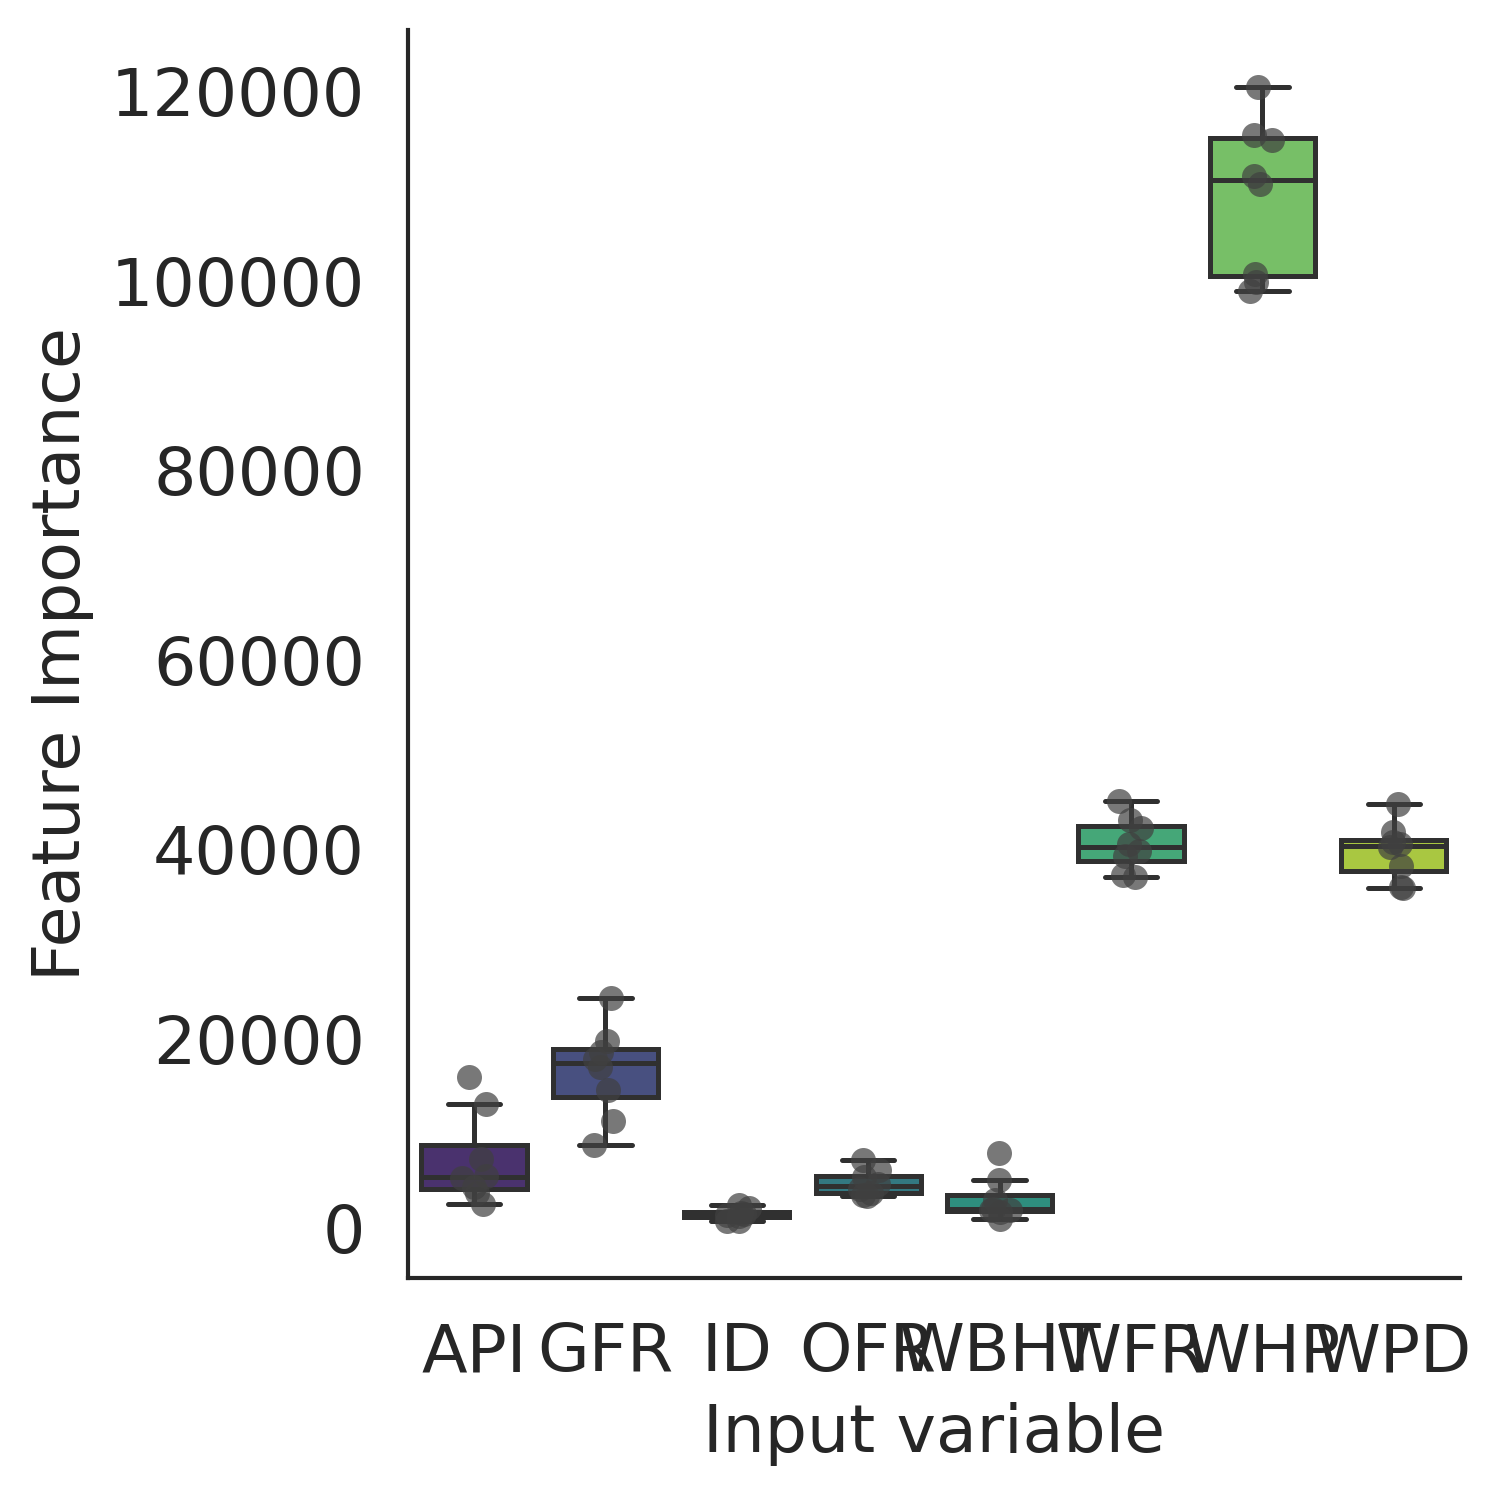
\includegraphics[width=0.8\textwidth]{./img/f1__fi_bxp_Fedot.png}
    \caption{F1  Fi Bxp Fedot}
    \label{fig:f1--fi-bxp-fedot}
\end{figure}

\begin{figure}[htbp]
    \centering
    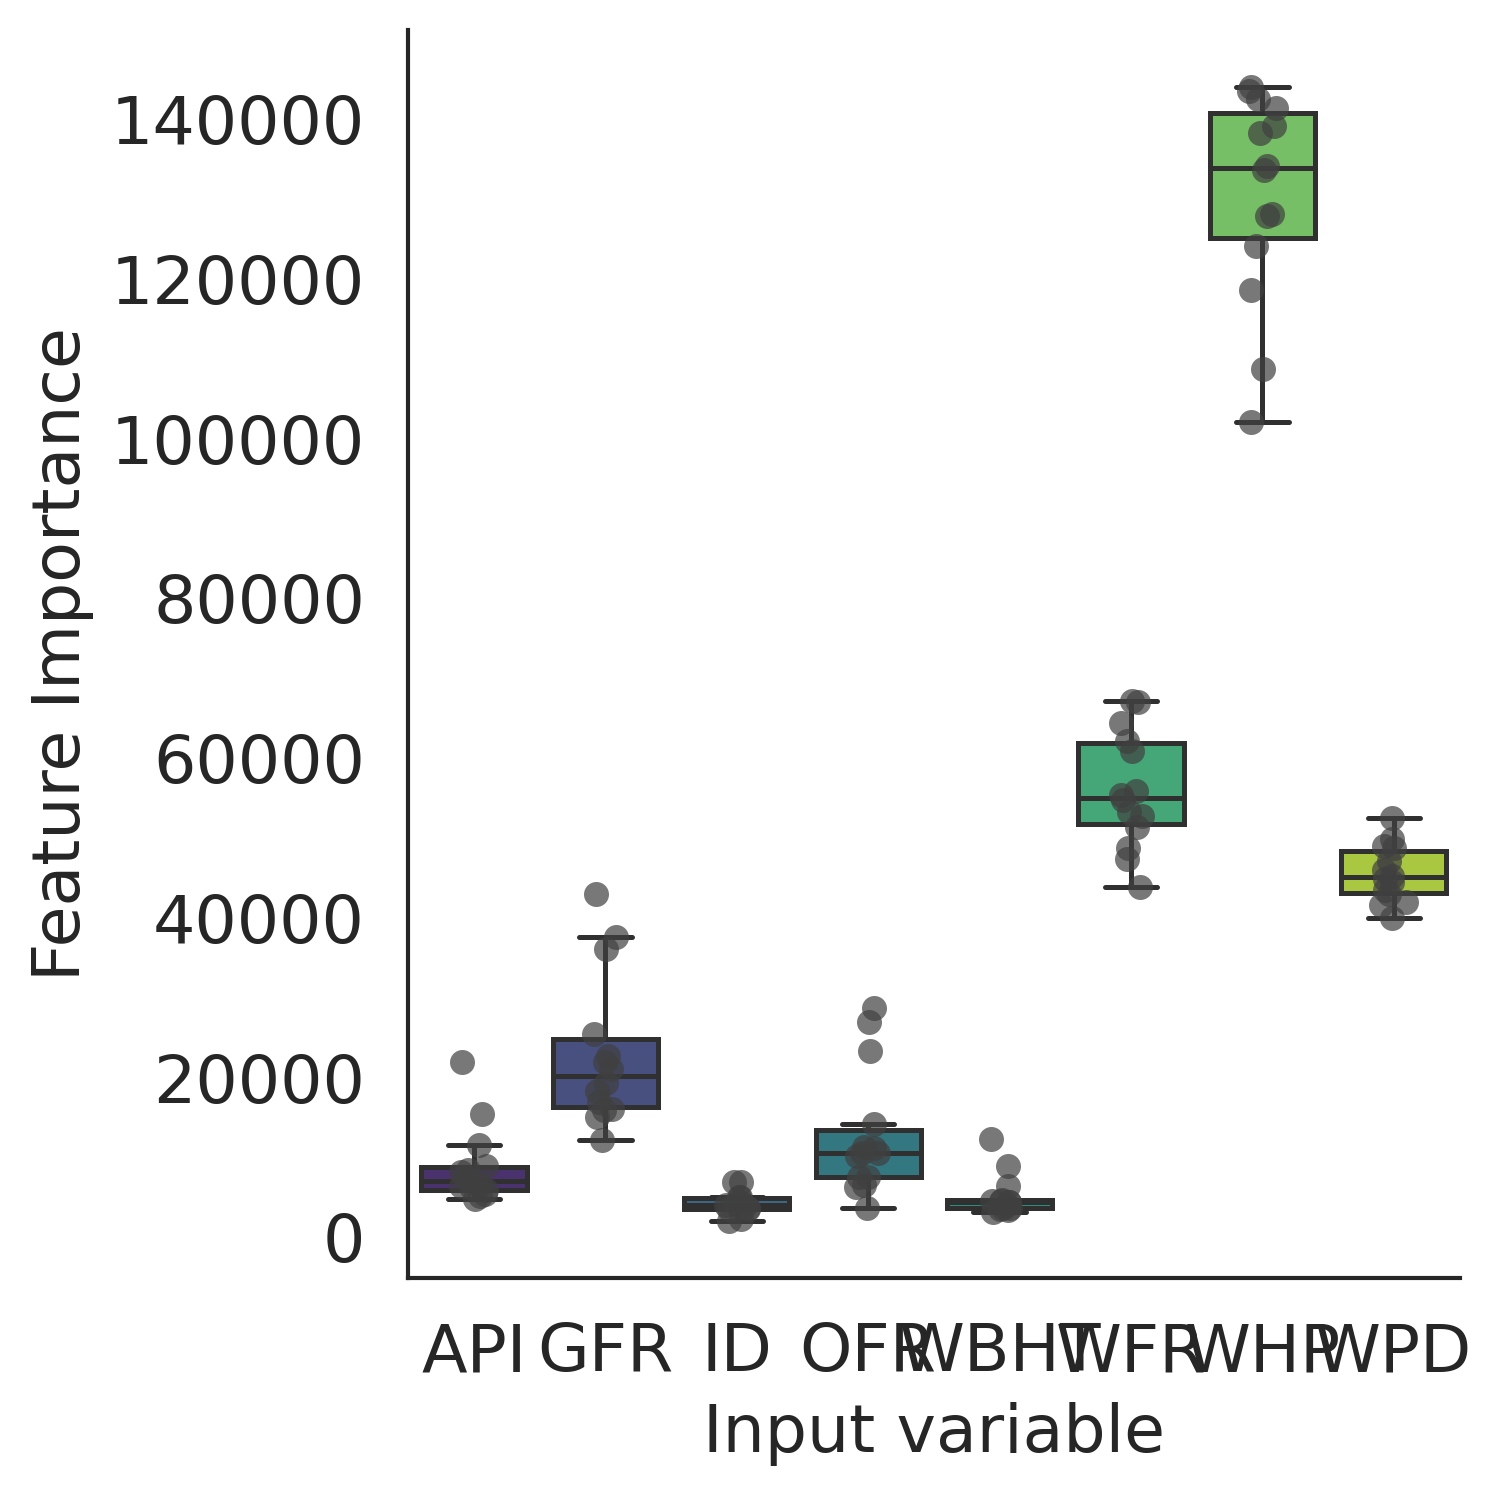
\includegraphics[width=0.8\textwidth]{./img/f1__fi_bxp_H2O.png}
    \caption{F1  Fi Bxp H2O}
    \label{fig:f1--fi-bxp-h2o}
\end{figure}

\begin{figure}[htbp]
    \centering
    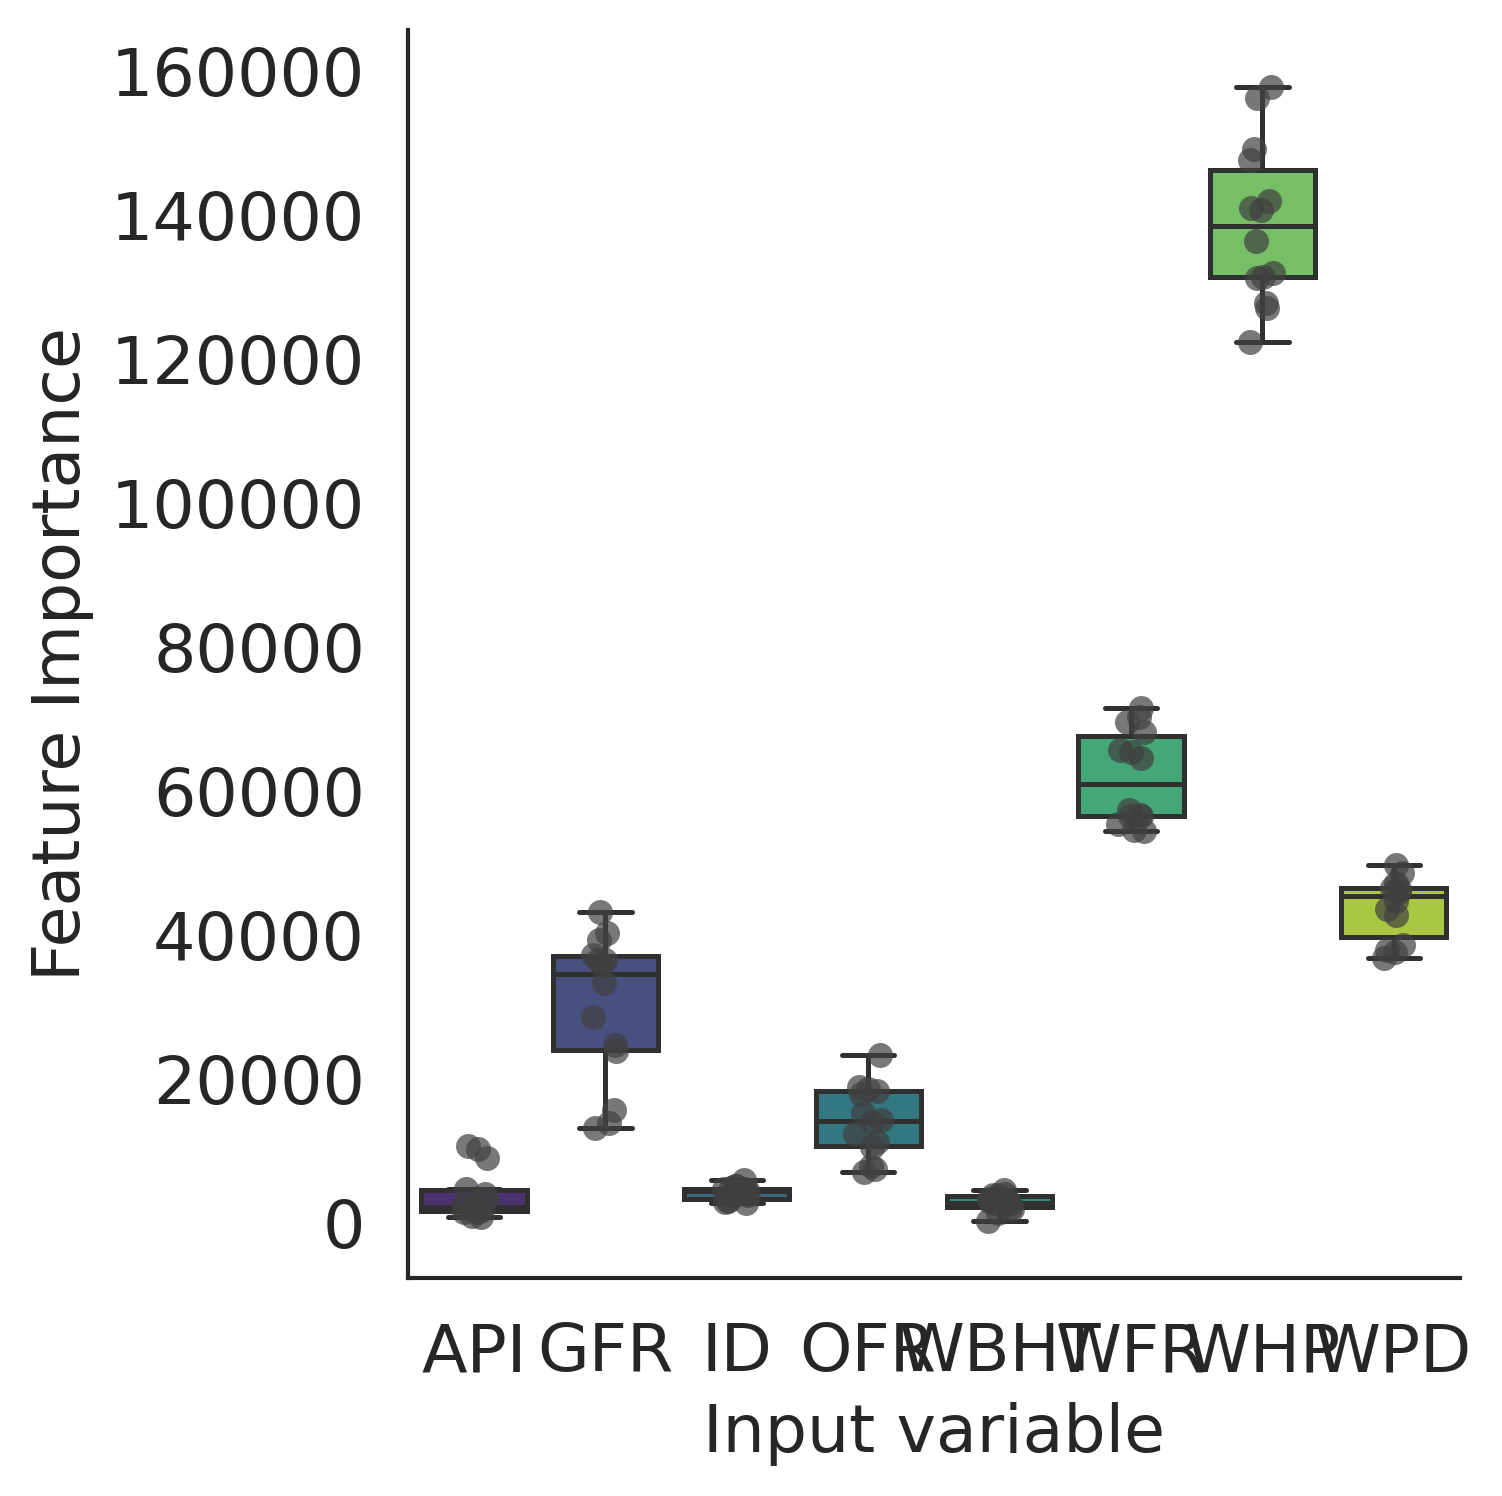
\includegraphics[width=0.8\textwidth]{./img/f1__fi_bxp_TPOT.png}
    \caption{F1  Fi Bxp Tpot}
    \label{fig:f1--fi-bxp-tpot}
\end{figure}

\begin{figure}[htbp]
    \centering
    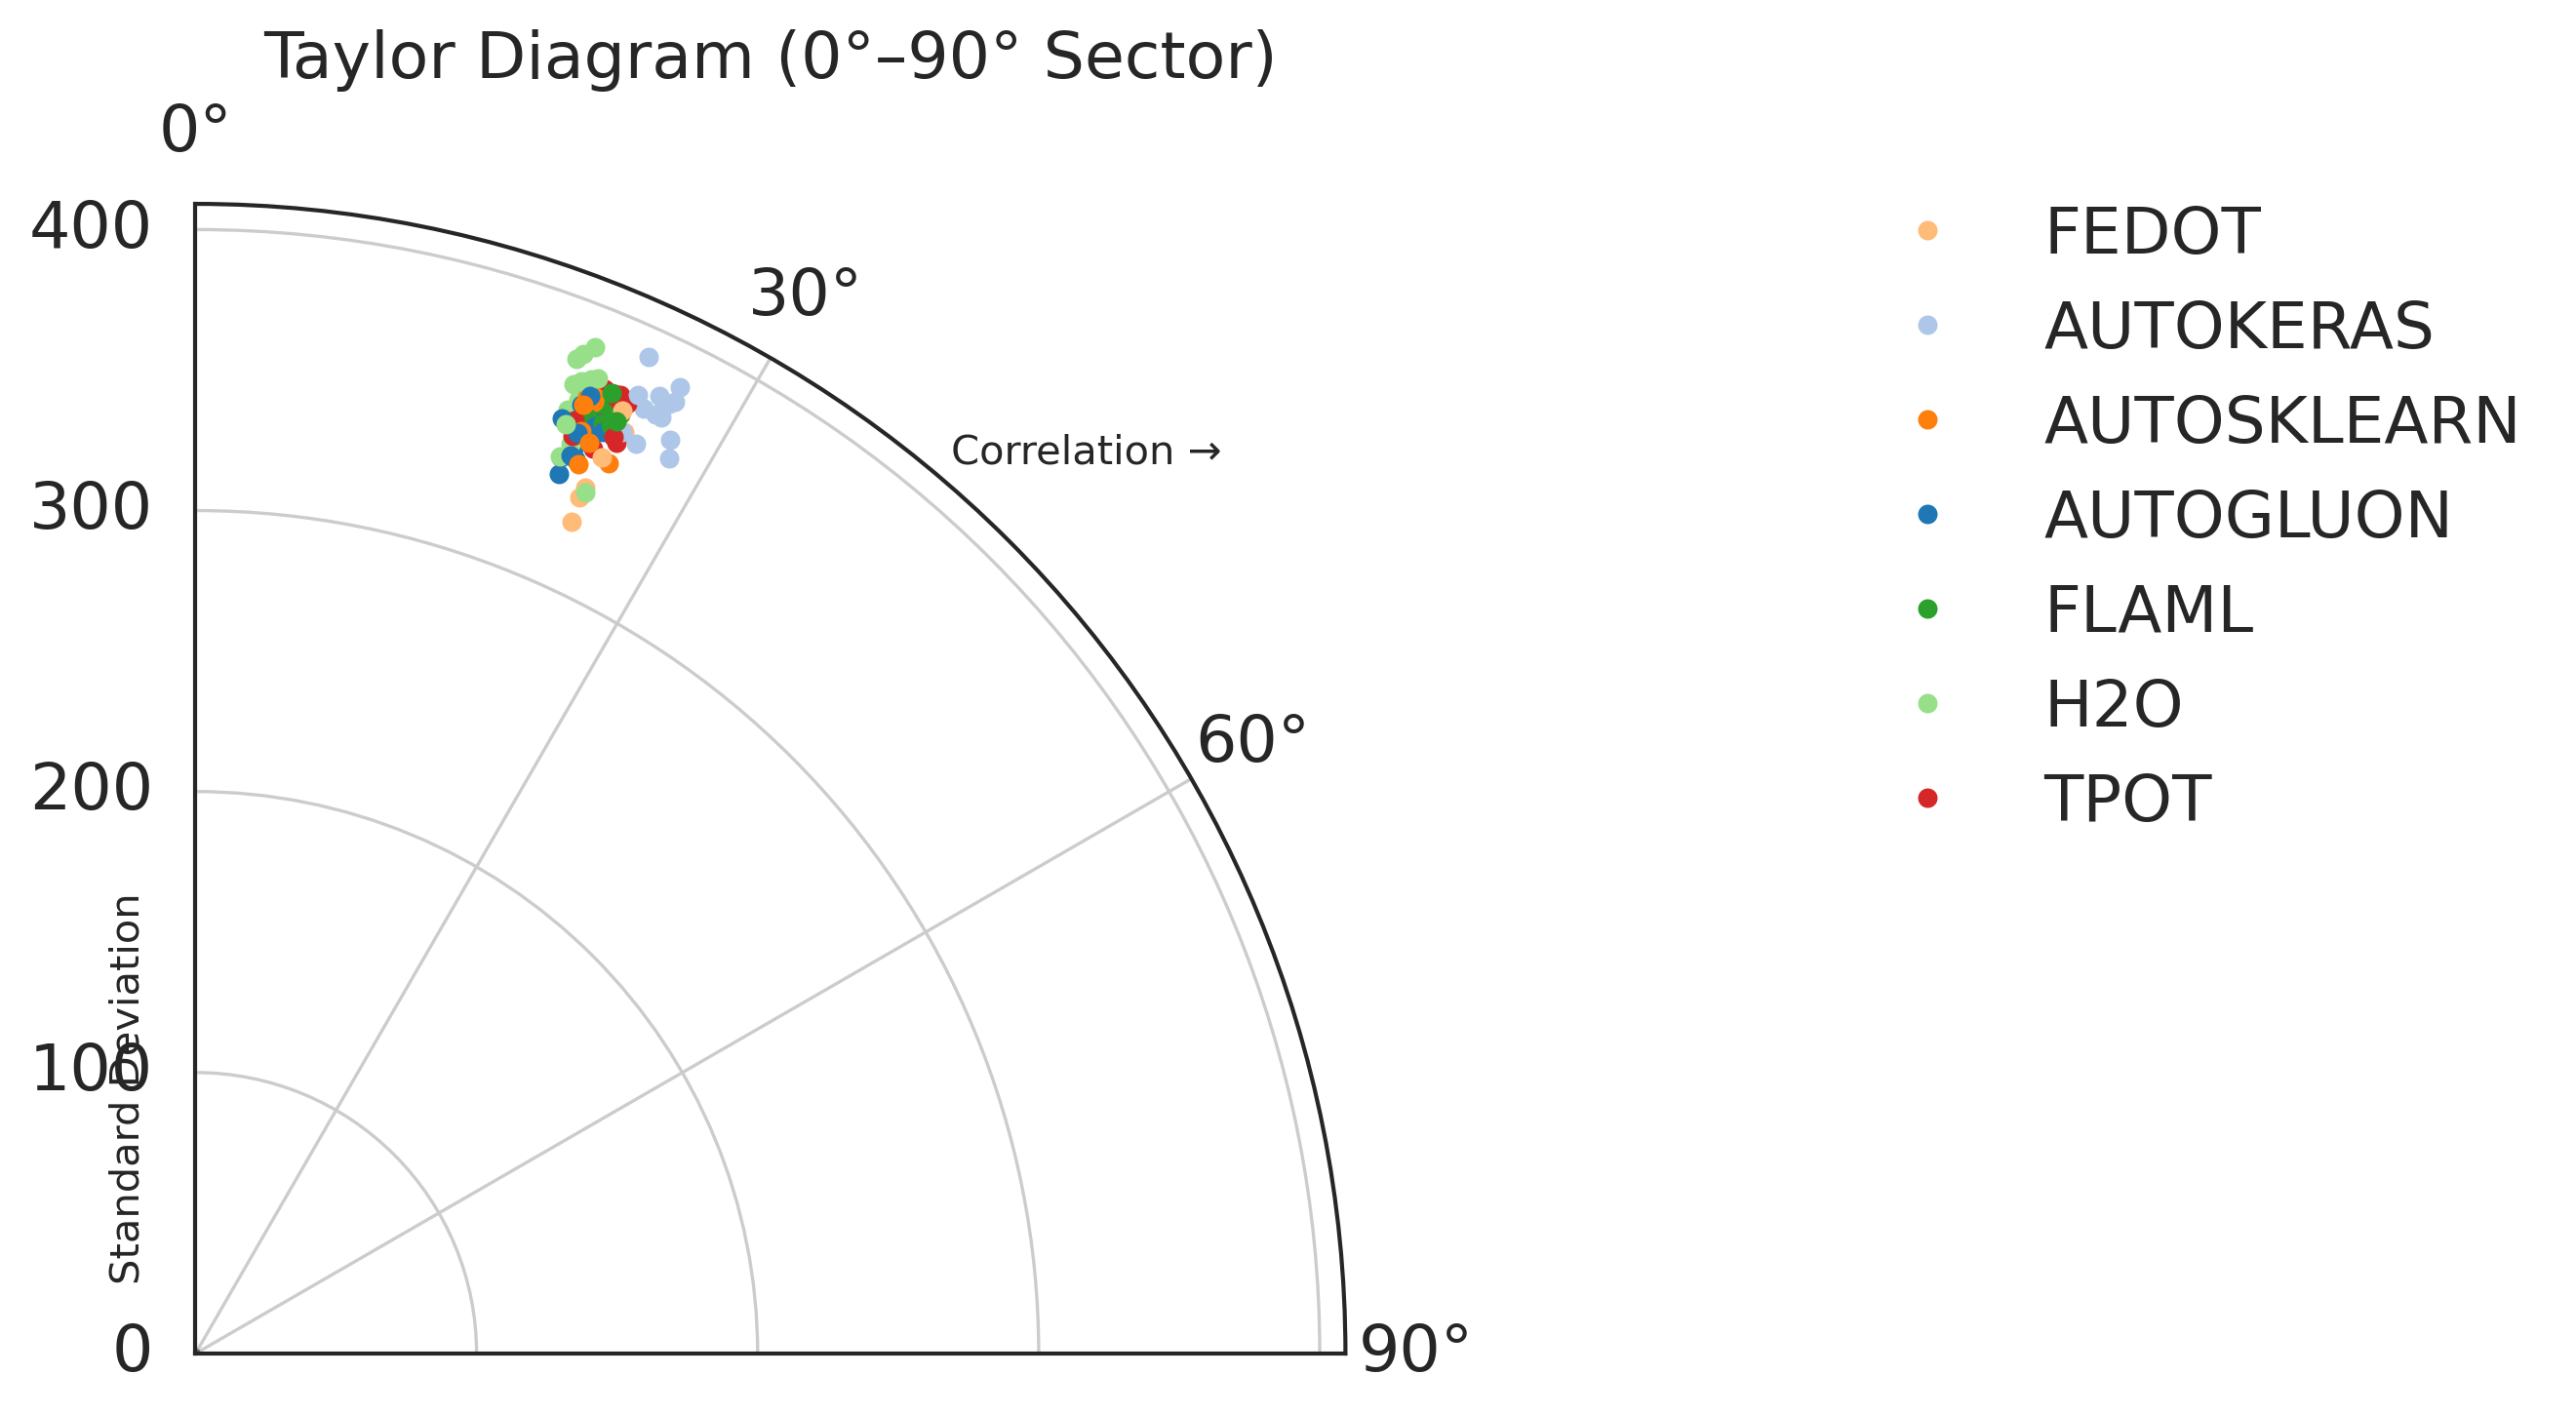
\includegraphics[width=0.8\textwidth]{./img/f1__taylor.png}
    \caption{F1  Taylor}
    \label{fig:f1--taylor}
\end{figure}

\begin{figure}[htbp]
    \centering
    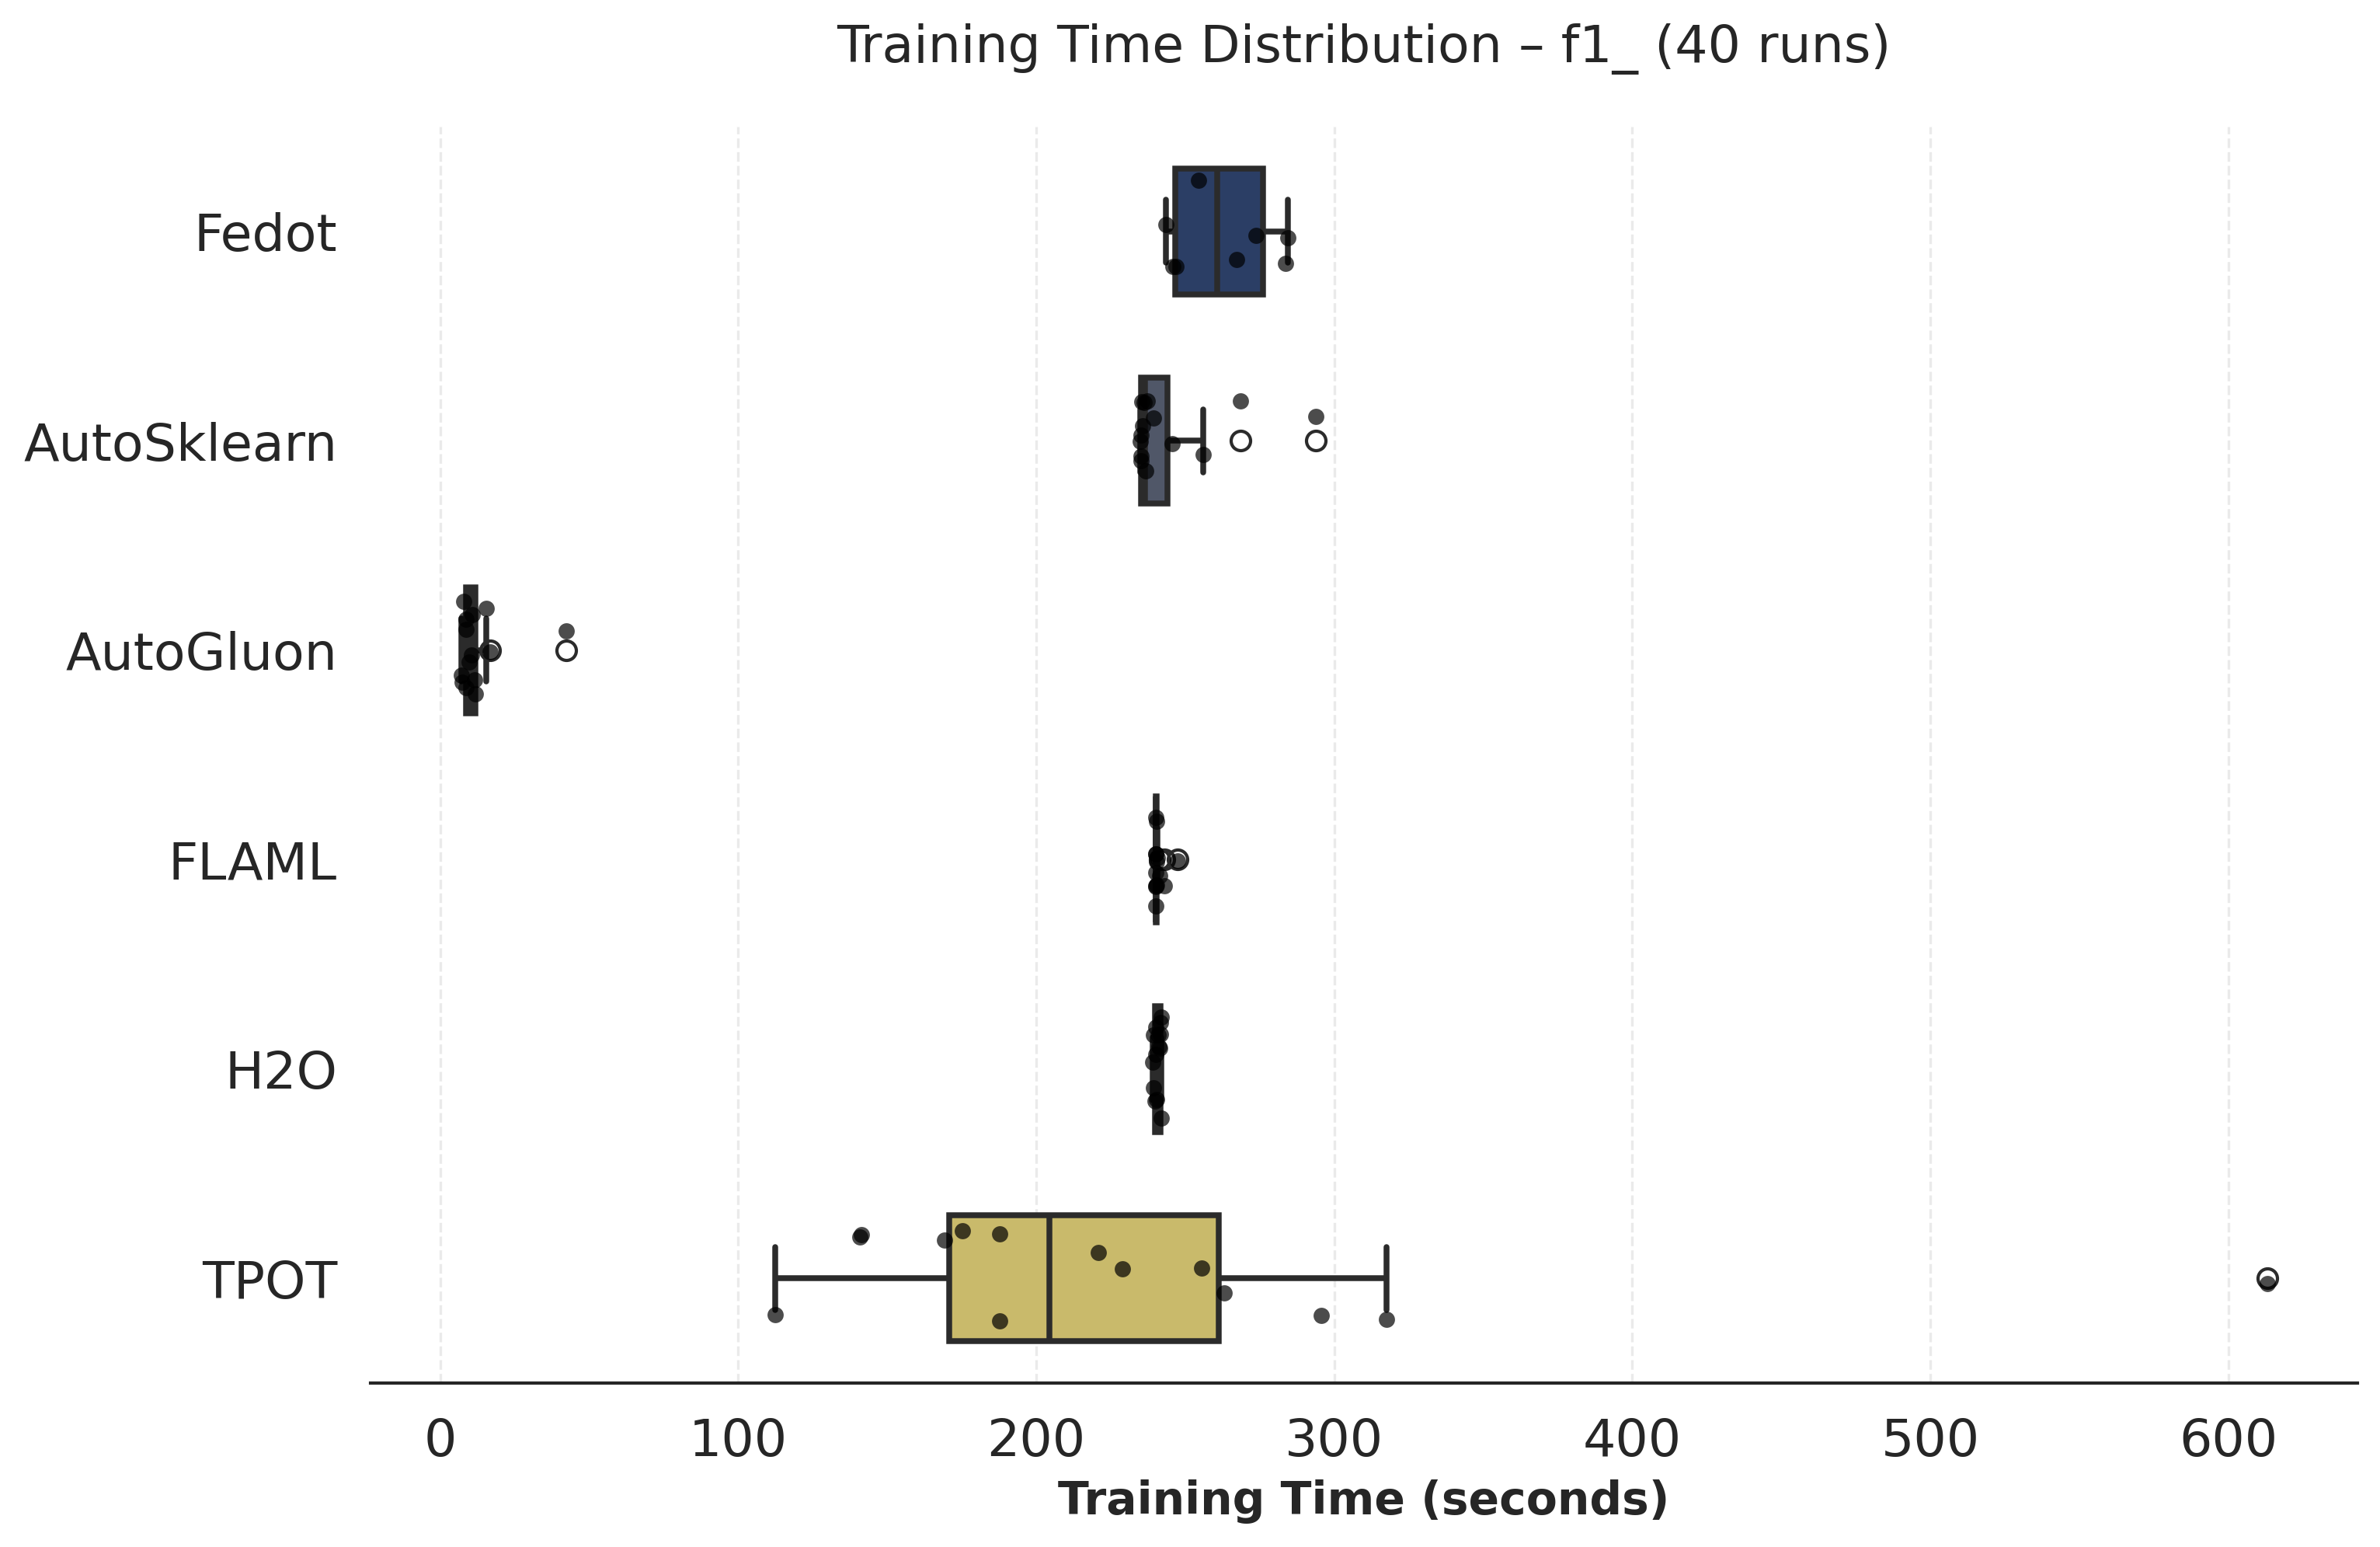
\includegraphics[width=0.8\textwidth]{./img/f1__time_boxplot_horizontal.png}
    \caption{F1  Time Boxplot Horizontal}
    \label{fig:f1--time-boxplot-horizontal}
\end{figure}

\begin{figure}[htbp]
    \centering
    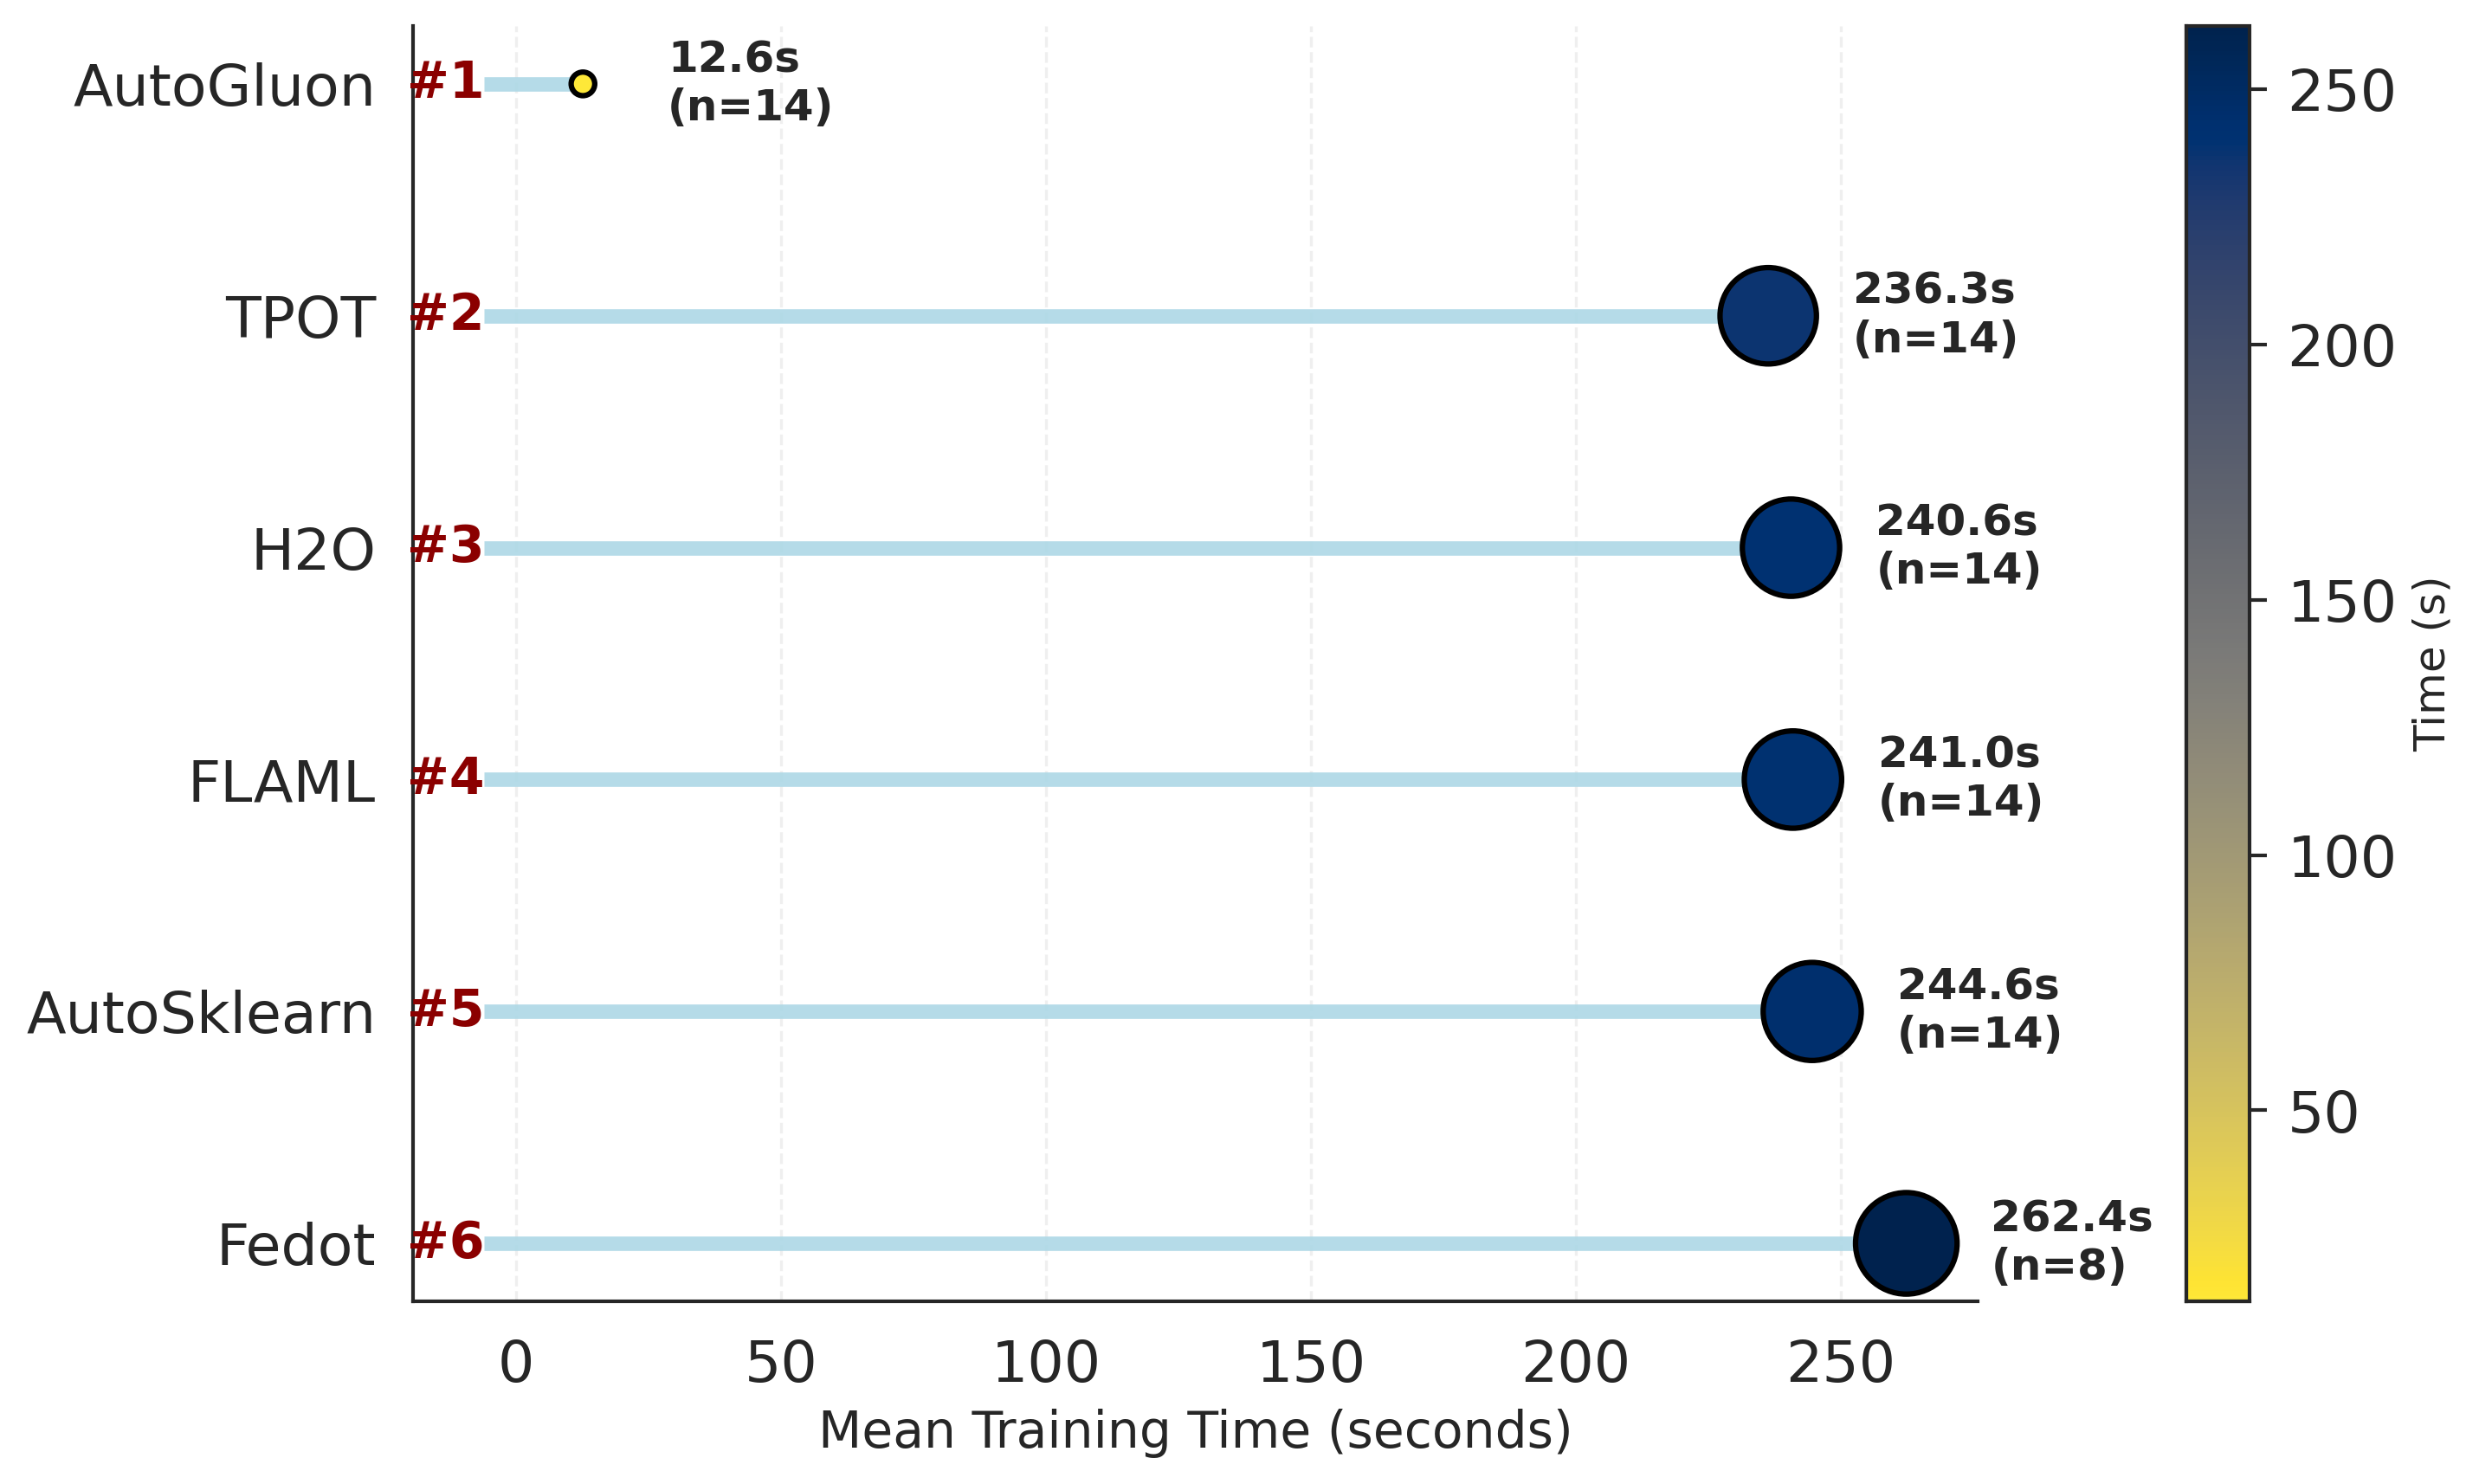
\includegraphics[width=0.8\textwidth]{./img/f1__time_lollipop_ranking.png}
    \caption{F1  Time Lollipop Ranking}
    \label{fig:f1--time-lollipop-ranking}
\end{figure}

